% This must be in the first 5 lines to tell arXiv to use pdfLaTeX.
\pdfoutput=1
\documentclass[11pt]{article}

% =====================================================================
% DRAFT (2026-09-27), story version: what synthetic PII benchmarks rank.
% Every number comes from generated/ (scripts/audit_paper_tables.py and
% scripts/rare_pii_tables.py); nothing is typed by hand.
%   "--"            = not measured yet (hand check of the probes).
%   \pending{...}   = text written only once those numbers exist.
% Previous version: acl2023_pii_audit_v1_before_story.tex.
% =====================================================================

\usepackage[review]{acl2023}

\usepackage{times}
\usepackage{latexsym}
\usepackage[T1]{fontenc}
\usepackage[utf8]{inputenc}
\usepackage{microtype}
\usepackage{inconsolata}

\usepackage{graphicx}
\usepackage{amsmath}
\usepackage{amssymb}
\usepackage{booktabs}
\usepackage{placeins}   % \FloatBarrier: main-text tables stay before Limitations

\setcounter{secnumdepth}{2}

\newcommand{\na}{--}
% generated by scripts/rare_pii_tables.py -- do not edit
\newcommand{\nSeeds}{two or three}
\newcommand{\seedList}{42 and 1337 for (a) and (c); 42, 1337 and 2024 for (b)}
\newcommand{\tuneGrid}{$\{0.50,0.55,\dots,0.90\}$}
          % \nSeeds, \seedList, \tuneGrid   (rare_pii_tables.py)
% generated by scripts/audit_paper_tables.py -- do not edit
\newcommand{\au}[2]{\csname au@#1@#2\endcsname}
\newcommand{\sn}[2]{\csname sn@#1@#2\endcsname}
\newcommand{\rt}[1]{\csname rt@#1\endcsname}
\newcommand{\zs}[2]{\csname zs@#1@#2\endcsname}
\newcommand{\os}[2]{\csname os@#1@#2\endcsname}
\newcommand{\ab}[1]{\csname ab@#1\endcsname}
\newcommand{\af}[1]{\csname af@#1\endcsname}
\newcommand{\tm}[1]{\csname tm@#1\endcsname}
\newcommand{\rv}[1]{\csname rv@#1\endcsname}
\newcommand{\lp}[1]{\csname lp@#1\endcsname}
\newcommand{\nm}[1]{\csname nm@#1\endcsname}
\newcommand{\cb}[1]{\csname cb@#1\endcsname}
\expandafter\def\csname au@privy@types\endcsname{17}
\expandafter\def\csname au@privy@train\endcsname{49{,}922}
\expandafter\def\csname au@privy@test\endcsname{5{,}000}
\expandafter\def\csname au@privy@lttwenty\endcsname{0}
\expandafter\def\csname au@privy@raremin\endcsname{129}
\expandafter\def\csname au@privy@raremed\endcsname{136}
\expandafter\def\csname au@privy@tmplleak\endcsname{0.2}
\expandafter\def\csname au@privy@exactdup\endcsname{0.04}
\expandafter\def\csname au@privy@valseen\endcsname{50.4}
\expandafter\def\csname au@privy@cnm\endcsname{0.3}
\expandafter\def\csname au@privy@uin\endcsname{0.0}
\expandafter\def\csname au@privy@uout\endcsname{0.0}
\expandafter\def\csname au@privy@uhits\endcsname{0}
\expandafter\def\csname au@privy@slotdocs\endcsname{0.00}
\expandafter\def\csname au@privy@slotdocsn\endcsname{0}
\expandafter\def\csname au@privy@nullvals\endcsname{0}
\expandafter\def\csname au@privy@markupvals\endcsname{0}
\expandafter\def\csname au@privy@badvals\endcsname{0.00}
\expandafter\def\csname au@privy@offset\endcsname{0.00}
\expandafter\def\csname au@privy@offsetn\endcsname{0}
\expandafter\def\csname au@privy@overlap\endcsname{0.00}
\expandafter\def\csname au@privy@iaa\endcsname{\na}
\expandafter\def\csname au@privy@iaaspan\endcsname{\na}
\expandafter\def\csname au@privy@iaapairs\endcsname{\na}
\expandafter\def\csname au@privy@iaadocs\endcsname{\na}
\expandafter\def\csname au@privy@recseen\endcsname{99.8}
\expandafter\def\csname au@privy@recnovel\endcsname{99.4}
\expandafter\def\csname au@pii_500k@types\endcsname{20}
\expandafter\def\csname au@pii_500k@train\endcsname{49{,}998}
\expandafter\def\csname au@pii_500k@test\endcsname{4{,}999}
\expandafter\def\csname au@pii_500k@lttwenty\endcsname{0}
\expandafter\def\csname au@pii_500k@raremin\endcsname{110}
\expandafter\def\csname au@pii_500k@raremed\endcsname{139}
\expandafter\def\csname au@pii_500k@tmplleak\endcsname{1.6}
\expandafter\def\csname au@pii_500k@exactdup\endcsname{0.56}
\expandafter\def\csname au@pii_500k@valseen\endcsname{28.6}
\expandafter\def\csname au@pii_500k@cnm\endcsname{7.2}
\expandafter\def\csname au@pii_500k@uin\endcsname{0.0}
\expandafter\def\csname au@pii_500k@uout\endcsname{0.0}
\expandafter\def\csname au@pii_500k@uhits\endcsname{0}
\expandafter\def\csname au@pii_500k@slotdocs\endcsname{0.48}
\expandafter\def\csname au@pii_500k@slotdocsn\endcsname{24}
\expandafter\def\csname au@pii_500k@nullvals\endcsname{0}
\expandafter\def\csname au@pii_500k@markupvals\endcsname{0}
\expandafter\def\csname au@pii_500k@badvals\endcsname{0.00}
\expandafter\def\csname au@pii_500k@offset\endcsname{0.00}
\expandafter\def\csname au@pii_500k@offsetn\endcsname{0}
\expandafter\def\csname au@pii_500k@overlap\endcsname{0.00}
\expandafter\def\csname au@pii_500k@iaa\endcsname{\na}
\expandafter\def\csname au@pii_500k@iaaspan\endcsname{\na}
\expandafter\def\csname au@pii_500k@iaapairs\endcsname{\na}
\expandafter\def\csname au@pii_500k@iaadocs\endcsname{\na}
\expandafter\def\csname au@pii_500k@slota\endcsname{\texttt{[LANGUAGEPLACEHOLDER\_\#]}}
\expandafter\def\csname au@pii_500k@slotan\endcsname{11}
\expandafter\def\csname au@pii_500k@slotb\endcsname{\texttt{[AMOUNTPLACEHOLDER\_\#]}}
\expandafter\def\csname au@pii_500k@slotbn\endcsname{5}
\expandafter\def\csname au@pii_500k@slotc\endcsname{\texttt{[ORGANISATIONPLACEHOLDER\_\#]}}
\expandafter\def\csname au@pii_500k@slotcn\endcsname{4}
\expandafter\def\csname au@pii_500k@recseen\endcsname{92.0}
\expandafter\def\csname au@pii_500k@recnovel\endcsname{88.5}
\expandafter\def\csname au@kiji@types\endcsname{28}
\expandafter\def\csname au@kiji@train\endcsname{43{,}845}
\expandafter\def\csname au@kiji@test\endcsname{5{,}000}
\expandafter\def\csname au@kiji@lttwenty\endcsname{2}
\expandafter\def\csname au@kiji@raremin\endcsname{4}
\expandafter\def\csname au@kiji@raremed\endcsname{576}
\expandafter\def\csname au@kiji@tmplleak\endcsname{2.8}
\expandafter\def\csname au@kiji@exactdup\endcsname{0.00}
\expandafter\def\csname au@kiji@valseen\endcsname{83.7}
\expandafter\def\csname au@kiji@cnm\endcsname{5.8}
\expandafter\def\csname au@kiji@uin\endcsname{2.0}
\expandafter\def\csname au@kiji@uout\endcsname{0.0}
\expandafter\def\csname au@kiji@uhits\endcsname{10}
\expandafter\def\csname au@kiji@slotdocs\endcsname{0.00}
\expandafter\def\csname au@kiji@slotdocsn\endcsname{0}
\expandafter\def\csname au@kiji@nullvals\endcsname{0}
\expandafter\def\csname au@kiji@markupvals\endcsname{0}
\expandafter\def\csname au@kiji@badvals\endcsname{0.00}
\expandafter\def\csname au@kiji@offset\endcsname{0.00}
\expandafter\def\csname au@kiji@offsetn\endcsname{0}
\expandafter\def\csname au@kiji@overlap\endcsname{1.70}
\expandafter\def\csname au@kiji@iaa\endcsname{\na}
\expandafter\def\csname au@kiji@iaaspan\endcsname{\na}
\expandafter\def\csname au@kiji@iaapairs\endcsname{\na}
\expandafter\def\csname au@kiji@iaadocs\endcsname{\na}
\expandafter\def\csname au@kiji@recseen\endcsname{93.3}
\expandafter\def\csname au@kiji@recnovel\endcsname{90.9}
\expandafter\def\csname au@gretel@types\endcsname{42}
\expandafter\def\csname au@gretel@train\endcsname{50{,}000}
\expandafter\def\csname au@gretel@test\endcsname{5{,}000}
\expandafter\def\csname au@gretel@lttwenty\endcsname{2}
\expandafter\def\csname au@gretel@raremin\endcsname{2}
\expandafter\def\csname au@gretel@raremed\endcsname{66}
\expandafter\def\csname au@gretel@tmplleak\endcsname{4.2}
\expandafter\def\csname au@gretel@exactdup\endcsname{0.00}
\expandafter\def\csname au@gretel@valseen\endcsname{14.1}
\expandafter\def\csname au@gretel@cnm\endcsname{4.1}
\expandafter\def\csname au@gretel@uin\endcsname{1.0}
\expandafter\def\csname au@gretel@uout\endcsname{0.0}
\expandafter\def\csname au@gretel@uhits\endcsname{5}
\expandafter\def\csname au@gretel@slotdocs\endcsname{0.06}
\expandafter\def\csname au@gretel@slotdocsn\endcsname{3}
\expandafter\def\csname au@gretel@nullvals\endcsname{0}
\expandafter\def\csname au@gretel@markupvals\endcsname{0}
\expandafter\def\csname au@gretel@badvals\endcsname{0.00}
\expandafter\def\csname au@gretel@offset\endcsname{0.00}
\expandafter\def\csname au@gretel@offsetn\endcsname{0}
\expandafter\def\csname au@gretel@overlap\endcsname{0.00}
\expandafter\def\csname au@gretel@iaa\endcsname{\na}
\expandafter\def\csname au@gretel@iaaspan\endcsname{\na}
\expandafter\def\csname au@gretel@iaapairs\endcsname{\na}
\expandafter\def\csname au@gretel@iaadocs\endcsname{\na}
\expandafter\def\csname au@gretel@slota\endcsname{\texttt{[AMOUNT]}}
\expandafter\def\csname au@gretel@slotan\endcsname{1}
\expandafter\def\csname au@gretel@slotb\endcsname{\texttt{[RATE]}}
\expandafter\def\csname au@gretel@slotbn\endcsname{1}
\expandafter\def\csname au@gretel@slotc\endcsname{\texttt{[TERMS]}}
\expandafter\def\csname au@gretel@slotcn\endcsname{1}
\expandafter\def\csname au@gretel@recseen\endcsname{91.2}
\expandafter\def\csname au@gretel@recnovel\endcsname{96.5}
\expandafter\def\csname au@nemotron@types\endcsname{55}
\expandafter\def\csname au@nemotron@train\endcsname{100{,}000}
\expandafter\def\csname au@nemotron@test\endcsname{100{,}000}
\expandafter\def\csname au@nemotron@lttwenty\endcsname{0}
\expandafter\def\csname au@nemotron@raremin\endcsname{1{,}302}
\expandafter\def\csname au@nemotron@raremed\endcsname{5{,}549}
\expandafter\def\csname au@nemotron@tmplleak\endcsname{0.0}
\expandafter\def\csname au@nemotron@exactdup\endcsname{0.00}
\expandafter\def\csname au@nemotron@valseen\endcsname{52.8}
\expandafter\def\csname au@nemotron@cnm\endcsname{1.8}
\expandafter\def\csname au@nemotron@uin\endcsname{0.3}
\expandafter\def\csname au@nemotron@uout\endcsname{0.0}
\expandafter\def\csname au@nemotron@uhits\endcsname{32}
\expandafter\def\csname au@nemotron@slotdocs\endcsname{0.01}
\expandafter\def\csname au@nemotron@slotdocsn\endcsname{11}
\expandafter\def\csname au@nemotron@nullvals\endcsname{31}
\expandafter\def\csname au@nemotron@markupvals\endcsname{12}
\expandafter\def\csname au@nemotron@badvals\endcsname{0.01}
\expandafter\def\csname au@nemotron@offset\endcsname{0.77}
\expandafter\def\csname au@nemotron@offsetn\endcsname{12{,}965}
\expandafter\def\csname au@nemotron@overlap\endcsname{0.01}
\expandafter\def\csname au@nemotron@iaa\endcsname{\na}
\expandafter\def\csname au@nemotron@iaaspan\endcsname{\na}
\expandafter\def\csname au@nemotron@iaapairs\endcsname{\na}
\expandafter\def\csname au@nemotron@iaadocs\endcsname{\na}
\expandafter\def\csname au@nemotron@slota\endcsname{\texttt{[STATE]}}
\expandafter\def\csname au@nemotron@slotan\endcsname{12}
\expandafter\def\csname au@nemotron@slotb\endcsname{\texttt{[COUNTY]}}
\expandafter\def\csname au@nemotron@slotbn\endcsname{9}
\expandafter\def\csname au@nemotron@slotc\endcsname{\texttt{[JPEG]}}
\expandafter\def\csname au@nemotron@slotcn\endcsname{2}
\expandafter\def\csname au@ai4privacy_300k@types\endcsname{28}
\expandafter\def\csname au@ai4privacy_300k@train\endcsname{177{,}677}
\expandafter\def\csname au@ai4privacy_300k@test\endcsname{47{,}728}
\expandafter\def\csname au@ai4privacy_300k@lttwenty\endcsname{1}
\expandafter\def\csname au@ai4privacy_300k@raremin\endcsname{17}
\expandafter\def\csname au@ai4privacy_300k@raremed\endcsname{10{,}498}
\expandafter\def\csname au@ai4privacy_300k@tmplleak\endcsname{0.0}
\expandafter\def\csname au@ai4privacy_300k@exactdup\endcsname{0.00}
\expandafter\def\csname au@ai4privacy_300k@valseen\endcsname{42.9}
\expandafter\def\csname au@ai4privacy_300k@cnm\endcsname{4.8}
\expandafter\def\csname au@ai4privacy_300k@uin\endcsname{1.3}
\expandafter\def\csname au@ai4privacy_300k@uout\endcsname{0.1}
\expandafter\def\csname au@ai4privacy_300k@uhits\endcsname{69}
\expandafter\def\csname au@ai4privacy_300k@slotdocs\endcsname{1.44}
\expandafter\def\csname au@ai4privacy_300k@slotdocsn\endcsname{687}
\expandafter\def\csname au@ai4privacy_300k@nullvals\endcsname{229}
\expandafter\def\csname au@ai4privacy_300k@markupvals\endcsname{132}
\expandafter\def\csname au@ai4privacy_300k@badvals\endcsname{0.11}
\expandafter\def\csname au@ai4privacy_300k@offset\endcsname{0.52}
\expandafter\def\csname au@ai4privacy_300k@offsetn\endcsname{7{,}812}
\expandafter\def\csname au@ai4privacy_300k@overlap\endcsname{0.68}
\expandafter\def\csname au@ai4privacy_300k@iaa\endcsname{\na}
\expandafter\def\csname au@ai4privacy_300k@iaaspan\endcsname{\na}
\expandafter\def\csname au@ai4privacy_300k@iaapairs\endcsname{\na}
\expandafter\def\csname au@ai4privacy_300k@iaadocs\endcsname{\na}
\expandafter\def\csname au@ai4privacy_300k@slota\endcsname{\texttt{DATE\_BG(}}
\expandafter\def\csname au@ai4privacy_300k@slotan\endcsname{47}
\expandafter\def\csname au@ai4privacy_300k@slotb\endcsname{\texttt{[LASTNAME\#\_A]}}
\expandafter\def\csname au@ai4privacy_300k@slotbn\endcsname{42}
\expandafter\def\csname au@ai4privacy_300k@slotc\endcsname{\texttt{{{\#}}}}
\expandafter\def\csname au@ai4privacy_300k@slotcn\endcsname{30}
\expandafter\def\csname au@ai4privacy_400k@types\endcsname{17}
\expandafter\def\csname au@ai4privacy_400k@train\endcsname{325{,}517}
\expandafter\def\csname au@ai4privacy_400k@test\endcsname{81{,}379}
\expandafter\def\csname au@ai4privacy_400k@lttwenty\endcsname{0}
\expandafter\def\csname au@ai4privacy_400k@raremin\endcsname{2{,}483}
\expandafter\def\csname au@ai4privacy_400k@raremed\endcsname{3{,}038}
\expandafter\def\csname au@ai4privacy_400k@tmplleak\endcsname{0.2}
\expandafter\def\csname au@ai4privacy_400k@exactdup\endcsname{0.04}
\expandafter\def\csname au@ai4privacy_400k@valseen\endcsname{28.3}
\expandafter\def\csname au@ai4privacy_400k@cnm\endcsname{3.4}
\expandafter\def\csname au@ai4privacy_400k@uin\endcsname{0.0}
\expandafter\def\csname au@ai4privacy_400k@uout\endcsname{12.2}
\expandafter\def\csname au@ai4privacy_400k@uhits\endcsname{995}
\expandafter\def\csname au@ai4privacy_400k@slotdocs\endcsname{9.32}
\expandafter\def\csname au@ai4privacy_400k@slotdocsn\endcsname{7{,}587}
\expandafter\def\csname au@ai4privacy_400k@nullvals\endcsname{25}
\expandafter\def\csname au@ai4privacy_400k@markupvals\endcsname{0}
\expandafter\def\csname au@ai4privacy_400k@badvals\endcsname{0.03}
\expandafter\def\csname au@ai4privacy_400k@offset\endcsname{0.00}
\expandafter\def\csname au@ai4privacy_400k@offsetn\endcsname{0}
\expandafter\def\csname au@ai4privacy_400k@overlap\endcsname{0.00}
\expandafter\def\csname au@ai4privacy_400k@iaa\endcsname{\na}
\expandafter\def\csname au@ai4privacy_400k@iaaspan\endcsname{\na}
\expandafter\def\csname au@ai4privacy_400k@iaapairs\endcsname{\na}
\expandafter\def\csname au@ai4privacy_400k@iaadocs\endcsname{\na}
\expandafter\def\csname au@ai4privacy_400k@slota\endcsname{\texttt{[IPV\#\_\#]}}
\expandafter\def\csname au@ai4privacy_400k@slotan\endcsname{5{,}774}
\expandafter\def\csname au@ai4privacy_400k@slotb\endcsname{\texttt{[CREDITCARDEXPIRYCREDITCARDCVV\_\#]}}
\expandafter\def\csname au@ai4privacy_400k@slotbn\endcsname{946}
\expandafter\def\csname au@ai4privacy_400k@slotc\endcsname{\texttt{[NAME\_\#]}}
\expandafter\def\csname au@ai4privacy_400k@slotcn\endcsname{166}
\expandafter\def\csname au@gretel_finance@types\endcsname{29}
\expandafter\def\csname au@gretel_finance@train\endcsname{50{,}346}
\expandafter\def\csname au@gretel_finance@test\endcsname{5{,}594}
\expandafter\def\csname au@gretel_finance@lttwenty\endcsname{0}
\expandafter\def\csname au@gretel_finance@raremin\endcsname{71}
\expandafter\def\csname au@gretel_finance@raremed\endcsname{136}
\expandafter\def\csname au@gretel_finance@tmplleak\endcsname{0.5}
\expandafter\def\csname au@gretel_finance@exactdup\endcsname{0.14}
\expandafter\def\csname au@gretel_finance@valseen\endcsname{62.2}
\expandafter\def\csname au@gretel_finance@cnm\endcsname{1.1}
\expandafter\def\csname au@gretel_finance@uin\endcsname{0.2}
\expandafter\def\csname au@gretel_finance@uout\endcsname{3.4}
\expandafter\def\csname au@gretel_finance@uhits\endcsname{20}
\expandafter\def\csname au@gretel_finance@slotdocs\endcsname{0.36}
\expandafter\def\csname au@gretel_finance@slotdocsn\endcsname{20}
\expandafter\def\csname au@gretel_finance@nullvals\endcsname{0}
\expandafter\def\csname au@gretel_finance@markupvals\endcsname{5}
\expandafter\def\csname au@gretel_finance@badvals\endcsname{0.01}
\expandafter\def\csname au@gretel_finance@offset\endcsname{\na}
\expandafter\def\csname au@gretel_finance@offsetn\endcsname{\na}
\expandafter\def\csname au@gretel_finance@overlap\endcsname{2.19}
\expandafter\def\csname au@gretel_finance@iaa\endcsname{\na}
\expandafter\def\csname au@gretel_finance@iaaspan\endcsname{\na}
\expandafter\def\csname au@gretel_finance@iaapairs\endcsname{\na}
\expandafter\def\csname au@gretel_finance@iaadocs\endcsname{\na}
\expandafter\def\csname au@gretel_finance@slota\endcsname{\texttt{[REDACTED]}}
\expandafter\def\csname au@gretel_finance@slotan\endcsname{23}
\expandafter\def\csname au@gretel_finance@slotb\endcsname{\texttt{[DATE]}}
\expandafter\def\csname au@gretel_finance@slotbn\endcsname{5}
\expandafter\def\csname au@gretel_finance@slotc\endcsname{\texttt{[BIDM]}}
\expandafter\def\csname au@gretel_finance@slotcn\endcsname{4}
\expandafter\def\csname au@tab@types\endcsname{8}
\expandafter\def\csname au@tab@train\endcsname{1{,}014}
\expandafter\def\csname au@tab@test\endcsname{127}
\expandafter\def\csname au@tab@lttwenty\endcsname{0}
\expandafter\def\csname au@tab@raremin\endcsname{218}
\expandafter\def\csname au@tab@raremed\endcsname{340}
\expandafter\def\csname au@tab@tmplleak\endcsname{0.0}
\expandafter\def\csname au@tab@exactdup\endcsname{0.00}
\expandafter\def\csname au@tab@valseen\endcsname{63.5}
\expandafter\def\csname au@tab@cnm\endcsname{1.8}
\expandafter\def\csname au@tab@uin\endcsname{0.0}
\expandafter\def\csname au@tab@uout\endcsname{0.0}
\expandafter\def\csname au@tab@uhits\endcsname{0}
\expandafter\def\csname au@tab@slotdocs\endcsname{0.00}
\expandafter\def\csname au@tab@slotdocsn\endcsname{0}
\expandafter\def\csname au@tab@nullvals\endcsname{0}
\expandafter\def\csname au@tab@markupvals\endcsname{0}
\expandafter\def\csname au@tab@badvals\endcsname{0.00}
\expandafter\def\csname au@tab@offset\endcsname{0.00}
\expandafter\def\csname au@tab@offsetn\endcsname{0}
\expandafter\def\csname au@tab@overlap\endcsname{0.24}
\expandafter\def\csname au@tab@iaa\endcsname{82.8}
\expandafter\def\csname au@tab@iaaspan\endcsname{84.7}
\expandafter\def\csname au@tab@iaapairs\endcsname{1{,}543}
\expandafter\def\csname au@tab@iaadocs\endcsname{105}
\expandafter\def\csname au@mapa@types\endcsname{5}
\expandafter\def\csname au@mapa@train\endcsname{\na}
\expandafter\def\csname au@mapa@test\endcsname{10{,}838}
\expandafter\def\csname au@mapa@lttwenty\endcsname{0}
\expandafter\def\csname au@mapa@raremin\endcsname{24}
\expandafter\def\csname au@mapa@raremed\endcsname{536}
\expandafter\def\csname au@mapa@tmplleak\endcsname{\na}
\expandafter\def\csname au@mapa@exactdup\endcsname{\na}
\expandafter\def\csname au@mapa@valseen\endcsname{\na}
\expandafter\def\csname au@mapa@cnm\endcsname{4.0}
\expandafter\def\csname au@mapa@uin\endcsname{0.0}
\expandafter\def\csname au@mapa@uout\endcsname{0.1}
\expandafter\def\csname au@mapa@uhits\endcsname{1}
\expandafter\def\csname au@mapa@slotdocs\endcsname{0.00}
\expandafter\def\csname au@mapa@slotdocsn\endcsname{0}
\expandafter\def\csname au@mapa@nullvals\endcsname{0}
\expandafter\def\csname au@mapa@markupvals\endcsname{0}
\expandafter\def\csname au@mapa@badvals\endcsname{0.00}
\expandafter\def\csname au@mapa@offset\endcsname{\na}
\expandafter\def\csname au@mapa@offsetn\endcsname{\na}
\expandafter\def\csname au@mapa@overlap\endcsname{0.00}
\expandafter\def\csname au@mapa@iaa\endcsname{\na}
\expandafter\def\csname au@mapa@iaaspan\endcsname{\na}
\expandafter\def\csname au@mapa@iaapairs\endcsname{\na}
\expandafter\def\csname au@mapa@iaadocs\endcsname{\na}
\expandafter\def\csname au@gretel_finance@digitname\endcsname{288}
\expandafter\def\csname au@all@valseenmin\endcsname{14.1}
\expandafter\def\csname au@all@valseenmax\endcsname{83.7}
\expandafter\def\csname au@all@tmplleakmax\endcsname{4.2}
\expandafter\def\csname sn@V0@a\endcsname{86.10}
\expandafter\def\csname sn@V0@b\endcsname{87.19}
\expandafter\def\csname sn@V0@c\endcsname{87.64}
\expandafter\def\csname sn@V0@ba\endcsname{+1.09}
\expandafter\def\csname sn@V0@bap\endcsname{0.016}
\expandafter\def\csname sn@V0@ban\endcsname{7/8}
\expandafter\def\csname sn@V0@cb\endcsname{+0.45}
\expandafter\def\csname sn@V0@cbp\endcsname{0.117}
\expandafter\def\csname sn@V0@cbn\endcsname{5/8}
\expandafter\def\csname sn@V0@shift\endcsname{0.0}
\expandafter\def\csname sn@V1-10@a\endcsname{91.18}
\expandafter\def\csname sn@V1-10@b\endcsname{92.31}
\expandafter\def\csname sn@V1-10@c\endcsname{92.36}
\expandafter\def\csname sn@V1-10@ba\endcsname{+1.13}
\expandafter\def\csname sn@V1-10@bap\endcsname{0.016}
\expandafter\def\csname sn@V1-10@ban\endcsname{7/8}
\expandafter\def\csname sn@V1-10@cb\endcsname{+0.05}
\expandafter\def\csname sn@V1-10@cbp\endcsname{0.750}
\expandafter\def\csname sn@V1-10@cbn\endcsname{4/8}
\expandafter\def\csname sn@V1-10@shift\endcsname{+5.1}
\expandafter\def\csname sn@V1-10@dropped\endcsname{4}
\expandafter\def\csname sn@V1-20@a\endcsname{91.18}
\expandafter\def\csname sn@V1-20@b\endcsname{92.31}
\expandafter\def\csname sn@V1-20@c\endcsname{92.36}
\expandafter\def\csname sn@V1-20@ba\endcsname{+1.13}
\expandafter\def\csname sn@V1-20@bap\endcsname{0.016}
\expandafter\def\csname sn@V1-20@ban\endcsname{7/8}
\expandafter\def\csname sn@V1-20@cb\endcsname{+0.05}
\expandafter\def\csname sn@V1-20@cbp\endcsname{0.750}
\expandafter\def\csname sn@V1-20@cbn\endcsname{4/8}
\expandafter\def\csname sn@V1-20@shift\endcsname{+5.1}
\expandafter\def\csname sn@V1-20@dropped\endcsname{4}
\expandafter\def\csname sn@V1-50@a\endcsname{91.95}
\expandafter\def\csname sn@V1-50@b\endcsname{92.83}
\expandafter\def\csname sn@V1-50@c\endcsname{92.91}
\expandafter\def\csname sn@V1-50@ba\endcsname{+0.87}
\expandafter\def\csname sn@V1-50@bap\endcsname{0.016}
\expandafter\def\csname sn@V1-50@ban\endcsname{7/8}
\expandafter\def\csname sn@V1-50@cb\endcsname{+0.09}
\expandafter\def\csname sn@V1-50@cbp\endcsname{0.461}
\expandafter\def\csname sn@V1-50@cbn\endcsname{4/8}
\expandafter\def\csname sn@V1-50@shift\endcsname{+5.6}
\expandafter\def\csname sn@V1-50@dropped\endcsname{10}
\expandafter\def\csname sn@V2@a\endcsname{82.81}
\expandafter\def\csname sn@V2@b\endcsname{84.27}
\expandafter\def\csname sn@V2@c\endcsname{84.68}
\expandafter\def\csname sn@V2@ba\endcsname{+1.46}
\expandafter\def\csname sn@V2@bap\endcsname{0.023}
\expandafter\def\csname sn@V2@ban\endcsname{7/8}
\expandafter\def\csname sn@V2@cb\endcsname{+0.41}
\expandafter\def\csname sn@V2@cbp\endcsname{0.133}
\expandafter\def\csname sn@V2@cbn\endcsname{6/8}
\expandafter\def\csname sn@V2@shift\endcsname{$-$2.9}
\expandafter\def\csname sn@V2@kijidrop\endcsname{32{,}464}
\expandafter\def\csname sn@V2@kijitotal\endcsname{38{,}785}
\expandafter\def\csname sn@V3@a\endcsname{90.59}
\expandafter\def\csname sn@V3@b\endcsname{91.75}
\expandafter\def\csname sn@V3@c\endcsname{92.15}
\expandafter\def\csname sn@V3@ba\endcsname{+1.16}
\expandafter\def\csname sn@V3@bap\endcsname{0.031}
\expandafter\def\csname sn@V3@ban\endcsname{6/8}
\expandafter\def\csname sn@V3@cb\endcsname{+0.40}
\expandafter\def\csname sn@V3@cbp\endcsname{0.188}
\expandafter\def\csname sn@V3@cbn\endcsname{4/8}
\expandafter\def\csname sn@V3@shift\endcsname{+4.6}
\expandafter\def\csname sn@V4@a\endcsname{86.10}
\expandafter\def\csname sn@V4@b\endcsname{87.20}
\expandafter\def\csname sn@V4@c\endcsname{87.66}
\expandafter\def\csname sn@V4@ba\endcsname{+1.10}
\expandafter\def\csname sn@V4@bap\endcsname{0.016}
\expandafter\def\csname sn@V4@ban\endcsname{7/8}
\expandafter\def\csname sn@V4@cb\endcsname{+0.45}
\expandafter\def\csname sn@V4@cbp\endcsname{0.117}
\expandafter\def\csname sn@V4@cbn\endcsname{5/8}
\expandafter\def\csname sn@V4@shift\endcsname{0.0}
\expandafter\def\csname sn@all@bamin\endcsname{+0.87}
\expandafter\def\csname sn@all@bamax\endcsname{+1.46}
\expandafter\def\csname sn@all@bapmax\endcsname{0.031}
\expandafter\def\csname sn@all@cbmin\endcsname{+0.05}
\expandafter\def\csname sn@all@cbmax\endcsname{+0.45}
\expandafter\def\csname sn@all@cbpmin\endcsname{0.117}
\expandafter\def\csname sn@V3@kijilargest\endcsname{7}
\expandafter\def\csname rt@ba\endcsname{+1.09}
\expandafter\def\csname rt@bap\endcsname{0.016}
\expandafter\def\csname rt@ban\endcsname{7/8}
\expandafter\def\csname rt@baup\endcsname{38}
\expandafter\def\csname rt@badown\endcsname{9}
\expandafter\def\csname rt@balabels\endcsname{54}
\expandafter\def\csname rt@bawil\endcsname{0.000}
\expandafter\def\csname rt@bamicro\endcsname{$-$0.15}
\expandafter\def\csname rt@bacilo\endcsname{+0.77}
\expandafter\def\csname rt@bacihi\endcsname{+1.43}
\expandafter\def\csname rt@cb\endcsname{+0.45}
\expandafter\def\csname rt@cbp\endcsname{0.117}
\expandafter\def\csname rt@cbn\endcsname{5/8}
\expandafter\def\csname rt@cbup\endcsname{17}
\expandafter\def\csname rt@cbdown\endcsname{25}
\expandafter\def\csname rt@cblabels\endcsname{54}
\expandafter\def\csname rt@cbwil\endcsname{0.941}
\expandafter\def\csname rt@cbmicro\endcsname{$-$0.02}
\expandafter\def\csname rt@cbcilo\endcsname{$-$0.08}
\expandafter\def\csname rt@cbcihi\endcsname{+0.80}
\expandafter\def\csname rt@ca\endcsname{+1.54}
\expandafter\def\csname rt@cap\endcsname{0.008}
\expandafter\def\csname rt@can\endcsname{8/8}
\expandafter\def\csname rt@caup\endcsname{40}
\expandafter\def\csname rt@cadown\endcsname{7}
\expandafter\def\csname rt@calabels\endcsname{54}
\expandafter\def\csname rt@cawil\endcsname{0.000}
\expandafter\def\csname rt@camicro\endcsname{$-$0.17}
\expandafter\def\csname rt@cacilo\endcsname{+0.90}
\expandafter\def\csname rt@cacihi\endcsname{+1.98}
\expandafter\def\csname rt@arare\endcsname{86.10}
\expandafter\def\csname rt@brare\endcsname{87.18}
\expandafter\def\csname rt@crare\endcsname{87.64}
\expandafter\def\csname rt@bmicromin\endcsname{89.6}
\expandafter\def\csname rt@bmicromax\endcsname{99.6}
\expandafter\def\csname rt@bsdmax\endcsname{0.32}
\expandafter\def\csname rt@bsdmin\endcsname{0.02}
\expandafter\def\csname rt@cgretelspread\endcsname{3.0}
\expandafter\def\csname rt@pindelta\endcsname{+33.3}
\expandafter\def\csname rt@cbnopin\endcsname{+0.05}
\expandafter\def\csname au@val@O@pct\endcsname{24}
\expandafter\def\csname au@val@O@lo\endcsname{20}
\expandafter\def\csname au@val@O@hi\endcsname{27}
\expandafter\def\csname au@val@O@samplepct\endcsname{50}
\expandafter\def\csname au@val@O@kappa\endcsname{1.00}
\expandafter\def\csname au@val@O@unan\endcsname{100}
\expandafter\def\csname au@val@O@nmaj\endcsname{100}
\expandafter\def\csname au@val@C@pct\endcsname{18}
\expandafter\def\csname au@val@C@lo\endcsname{11}
\expandafter\def\csname au@val@C@hi\endcsname{24}
\expandafter\def\csname au@val@C@samplepct\endcsname{21}
\expandafter\def\csname au@val@C@kappa\endcsname{0.84}
\expandafter\def\csname au@val@C@unan\endcsname{92}
\expandafter\def\csname au@val@C@nmaj\endcsname{457}
\expandafter\def\csname au@val@U@pct\endcsname{9}
\expandafter\def\csname au@val@U@lo\endcsname{6}
\expandafter\def\csname au@val@U@hi\endcsname{11}
\expandafter\def\csname au@val@U@samplepct\endcsname{48}
\expandafter\def\csname au@val@U@kappa\endcsname{0.94}
\expandafter\def\csname au@val@U@unan\endcsname{94}
\expandafter\def\csname au@val@U@nmaj\endcsname{168}
\expandafter\def\csname au@val@U@piipct\endcsname{98}
\expandafter\def\csname au@val@G@pct\endcsname{94}
\expandafter\def\csname au@val@G@lo\endcsname{92}
\expandafter\def\csname au@val@G@hi\endcsname{97}
\expandafter\def\csname au@val@G@samplepct\endcsname{88}
\expandafter\def\csname au@val@G@kappa\endcsname{0.96}
\expandafter\def\csname au@val@G@unan\endcsname{99}
\expandafter\def\csname au@val@G@nmaj\endcsname{230}
\expandafter\def\csname au@val@ai4privacy_300k@C@pct\endcsname{19}
\expandafter\def\csname au@val@ai4privacy_300k@C@est\endcsname{1{,}212}
\expandafter\def\csname au@val@ai4privacy_300k@G@pct\endcsname{58}
\expandafter\def\csname au@val@ai4privacy_300k@G@est\endcsname{898}
\expandafter\def\csname au@val@ai4privacy_300k@O@pct\endcsname{98}
\expandafter\def\csname au@val@ai4privacy_300k@O@est\endcsname{1{,}748}
\expandafter\def\csname au@val@ai4privacy_300k@U@pct\endcsname{92}
\expandafter\def\csname au@val@ai4privacy_300k@U@est\endcsname{63}
\expandafter\def\csname au@val@ai4privacy_300k@U@piipct\endcsname{98}
\expandafter\def\csname au@val@ai4privacy_400k@C@pct\endcsname{6}
\expandafter\def\csname au@val@ai4privacy_400k@C@est\endcsname{43}
\expandafter\def\csname au@val@ai4privacy_400k@G@pct\endcsname{100}
\expandafter\def\csname au@val@ai4privacy_400k@G@est\endcsname{10{,}319}
\expandafter\def\csname au@val@ai4privacy_400k@U@pct\endcsname{0}
\expandafter\def\csname au@val@ai4privacy_400k@U@est\endcsname{0}
\expandafter\def\csname au@val@ai4privacy_400k@U@piipct\endcsname{100}
\expandafter\def\csname au@val@gretel@C@pct\endcsname{8}
\expandafter\def\csname au@val@gretel@C@est\endcsname{7}
\expandafter\def\csname au@val@gretel@G@pct\endcsname{60}
\expandafter\def\csname au@val@gretel@G@est\endcsname{3}
\expandafter\def\csname au@val@gretel@U@pct\endcsname{40}
\expandafter\def\csname au@val@gretel@U@est\endcsname{2}
\expandafter\def\csname au@val@gretel@U@piipct\endcsname{40}
\expandafter\def\csname au@val@gretel_finance@C@pct\endcsname{35}
\expandafter\def\csname au@val@gretel_finance@C@est\endcsname{97}
\expandafter\def\csname au@val@gretel_finance@G@pct\endcsname{92}
\expandafter\def\csname au@val@gretel_finance@G@est\endcsname{59}
\expandafter\def\csname au@val@gretel_finance@U@pct\endcsname{5}
\expandafter\def\csname au@val@gretel_finance@U@est\endcsname{1}
\expandafter\def\csname au@val@gretel_finance@U@piipct\endcsname{45}
\expandafter\def\csname au@val@kiji@C@pct\endcsname{10}
\expandafter\def\csname au@val@kiji@C@est\endcsname{182}
\expandafter\def\csname au@val@kiji@U@pct\endcsname{80}
\expandafter\def\csname au@val@kiji@U@est\endcsname{8}
\expandafter\def\csname au@val@kiji@U@piipct\endcsname{80}
\expandafter\def\csname au@val@mapa@C@pct\endcsname{64}
\expandafter\def\csname au@val@mapa@C@est\endcsname{120}
\expandafter\def\csname au@val@mapa@U@pct\endcsname{0}
\expandafter\def\csname au@val@mapa@U@est\endcsname{0}
\expandafter\def\csname au@val@mapa@U@piipct\endcsname{0}
\expandafter\def\csname au@val@nemotron@C@pct\endcsname{18}
\expandafter\def\csname au@val@nemotron@C@est\endcsname{1{,}853}
\expandafter\def\csname au@val@nemotron@G@pct\endcsname{100}
\expandafter\def\csname au@val@nemotron@G@est\endcsname{60}
\expandafter\def\csname au@val@nemotron@O@pct\endcsname{2}
\expandafter\def\csname au@val@nemotron@O@est\endcsname{124}
\expandafter\def\csname au@val@nemotron@U@pct\endcsname{72}
\expandafter\def\csname au@val@nemotron@U@est\endcsname{23}
\expandafter\def\csname au@val@nemotron@U@piipct\endcsname{72}
\expandafter\def\csname au@val@pii_500k@C@pct\endcsname{6}
\expandafter\def\csname au@val@pii_500k@C@est\endcsname{10}
\expandafter\def\csname au@val@pii_500k@G@pct\endcsname{100}
\expandafter\def\csname au@val@pii_500k@G@est\endcsname{27}
\expandafter\def\csname au@val@privy@C@pct\endcsname{0}
\expandafter\def\csname au@val@privy@C@est\endcsname{0}
\expandafter\def\csname au@val@tab@C@pct\endcsname{32}
\expandafter\def\csname au@val@tab@C@est\endcsname{47}
\expandafter\def\csname au@val@pairmin\endcsname{0.79}
\expandafter\def\csname au@val@pairmax\endcsname{1.00}
\expandafter\def\csname au@val@unanall\endcsname{95}
\expandafter\def\csname au@all@sampled\endcsname{964}
\expandafter\def\csname zs@privy@rare\endcsname{55.9}
\expandafter\def\csname zs@privy@rarefloor\endcsname{55.9}
\expandafter\def\csname zs@privy@floorshift\endcsname{0.0}
\expandafter\def\csname zs@privy@micro\endcsname{47.3}
\expandafter\def\csname zs@privy@prec\endcsname{55.3}
\expandafter\def\csname zs@privy@precclean\endcsname{55.3}
\expandafter\def\csname zs@privy@fpflag\endcsname{0.0}
\expandafter\def\csname zs@privy@failed\endcsname{0}
\expandafter\def\csname zs@privy@didequal\endcsname{+9.7}
\expandafter\def\csname zs@privy@didmention\endcsname{+5.9}
\expandafter\def\csname zs@privy@didpos\endcsname{3/6}
\expandafter\def\csname zs@privy@didpooled\endcsname{+7.3}
\expandafter\def\csname zs@pii_500k@rare\endcsname{34.2}
\expandafter\def\csname zs@pii_500k@rarefloor\endcsname{34.2}
\expandafter\def\csname zs@pii_500k@floorshift\endcsname{0.0}
\expandafter\def\csname zs@pii_500k@micro\endcsname{55.6}
\expandafter\def\csname zs@pii_500k@prec\endcsname{60.4}
\expandafter\def\csname zs@pii_500k@precclean\endcsname{60.4}
\expandafter\def\csname zs@pii_500k@fpflag\endcsname{0.1}
\expandafter\def\csname zs@pii_500k@failed\endcsname{0}
\expandafter\def\csname zs@pii_500k@didequal\endcsname{$-$5.4}
\expandafter\def\csname zs@pii_500k@didmention\endcsname{$-$8.6}
\expandafter\def\csname zs@pii_500k@didpos\endcsname{1/9}
\expandafter\def\csname zs@pii_500k@didpooled\endcsname{+1.4}
\expandafter\def\csname zs@kiji@rare\endcsname{65.2}
\expandafter\def\csname zs@kiji@rarefloor\endcsname{72.7}
\expandafter\def\csname zs@kiji@floorshift\endcsname{+7.5}
\expandafter\def\csname zs@kiji@micro\endcsname{63.6}
\expandafter\def\csname zs@kiji@prec\endcsname{66.5}
\expandafter\def\csname zs@kiji@precclean\endcsname{66.5}
\expandafter\def\csname zs@kiji@fpflag\endcsname{0.1}
\expandafter\def\csname zs@kiji@failed\endcsname{0}
\expandafter\def\csname zs@kiji@didequal\endcsname{+2.4}
\expandafter\def\csname zs@kiji@didmention\endcsname{+3.7}
\expandafter\def\csname zs@kiji@didpos\endcsname{11/24}
\expandafter\def\csname zs@kiji@didpooled\endcsname{+12.4}
\expandafter\def\csname zs@gretel@rare\endcsname{37.2}
\expandafter\def\csname zs@gretel@rarefloor\endcsname{40.2}
\expandafter\def\csname zs@gretel@floorshift\endcsname{+3.0}
\expandafter\def\csname zs@gretel@micro\endcsname{57.6}
\expandafter\def\csname zs@gretel@prec\endcsname{59.6}
\expandafter\def\csname zs@gretel@precclean\endcsname{59.6}
\expandafter\def\csname zs@gretel@fpflag\endcsname{0.1}
\expandafter\def\csname zs@gretel@failed\endcsname{0}
\expandafter\def\csname zs@gretel@didequal\endcsname{$-$10.8}
\expandafter\def\csname zs@gretel@didmention\endcsname{$-$4.6}
\expandafter\def\csname zs@gretel@didpos\endcsname{0/5}
\expandafter\def\csname zs@gretel@didpooled\endcsname{+10.4}
\expandafter\def\csname zs@nemotron@rare\endcsname{78.8}
\expandafter\def\csname zs@nemotron@rarefloor\endcsname{78.8}
\expandafter\def\csname zs@nemotron@floorshift\endcsname{0.0}
\expandafter\def\csname zs@nemotron@micro\endcsname{77.8}
\expandafter\def\csname zs@nemotron@prec\endcsname{82.1}
\expandafter\def\csname zs@nemotron@precclean\endcsname{82.1}
\expandafter\def\csname zs@nemotron@fpflag\endcsname{0.1}
\expandafter\def\csname zs@nemotron@failed\endcsname{0}
\expandafter\def\csname zs@nemotron@didequal\endcsname{+1.0}
\expandafter\def\csname zs@nemotron@didmention\endcsname{$-$0.3}
\expandafter\def\csname zs@nemotron@didpos\endcsname{17/35}
\expandafter\def\csname zs@nemotron@didpooled\endcsname{+14.9}
\expandafter\def\csname zs@ai4privacy_300k@rare\endcsname{57.2}
\expandafter\def\csname zs@ai4privacy_300k@rarefloor\endcsname{57.2}
\expandafter\def\csname zs@ai4privacy_300k@floorshift\endcsname{0.0}
\expandafter\def\csname zs@ai4privacy_300k@micro\endcsname{63.9}
\expandafter\def\csname zs@ai4privacy_300k@prec\endcsname{66.8}
\expandafter\def\csname zs@ai4privacy_300k@precclean\endcsname{66.8}
\expandafter\def\csname zs@ai4privacy_300k@fpflag\endcsname{0.3}
\expandafter\def\csname zs@ai4privacy_300k@failed\endcsname{0}
\expandafter\def\csname zs@ai4privacy_300k@didequal\endcsname{$-$1.3}
\expandafter\def\csname zs@ai4privacy_300k@didmention\endcsname{$-$2.3}
\expandafter\def\csname zs@ai4privacy_300k@didpos\endcsname{4/14}
\expandafter\def\csname zs@ai4privacy_300k@didpooled\endcsname{$-$14.8}
\expandafter\def\csname zs@ai4privacy_400k@rare\endcsname{43.2}
\expandafter\def\csname zs@ai4privacy_400k@rarefloor\endcsname{43.2}
\expandafter\def\csname zs@ai4privacy_400k@floorshift\endcsname{0.0}
\expandafter\def\csname zs@ai4privacy_400k@micro\endcsname{46.9}
\expandafter\def\csname zs@ai4privacy_400k@prec\endcsname{38.6}
\expandafter\def\csname zs@ai4privacy_400k@precclean\endcsname{39.5}
\expandafter\def\csname zs@ai4privacy_400k@fpflag\endcsname{3.7}
\expandafter\def\csname zs@ai4privacy_400k@failed\endcsname{0}
\expandafter\def\csname zs@ai4privacy_400k@didequal\endcsname{+1.3}
\expandafter\def\csname zs@ai4privacy_400k@didmention\endcsname{+1.7}
\expandafter\def\csname zs@ai4privacy_400k@didpos\endcsname{3/6}
\expandafter\def\csname zs@ai4privacy_400k@didpooled\endcsname{+0.9}
\expandafter\def\csname zs@gretel_finance@rare\endcsname{27.2}
\expandafter\def\csname zs@gretel_finance@rarefloor\endcsname{27.2}
\expandafter\def\csname zs@gretel_finance@floorshift\endcsname{0.0}
\expandafter\def\csname zs@gretel_finance@micro\endcsname{44.8}
\expandafter\def\csname zs@gretel_finance@prec\endcsname{41.5}
\expandafter\def\csname zs@gretel_finance@precclean\endcsname{41.5}
\expandafter\def\csname zs@gretel_finance@fpflag\endcsname{0.1}
\expandafter\def\csname zs@gretel_finance@failed\endcsname{1}
\expandafter\def\csname zs@gretel_finance@didequal\endcsname{+5.1}
\expandafter\def\csname zs@gretel_finance@didmention\endcsname{+6.8}
\expandafter\def\csname zs@gretel_finance@didpos\endcsname{7/11}
\expandafter\def\csname zs@gretel_finance@didpooled\endcsname{+7.9}
\expandafter\def\csname zs@tab@rare\endcsname{27.9}
\expandafter\def\csname zs@tab@rarefloor\endcsname{27.9}
\expandafter\def\csname zs@tab@floorshift\endcsname{0.0}
\expandafter\def\csname zs@tab@micro\endcsname{57.6}
\expandafter\def\csname zs@tab@prec\endcsname{61.3}
\expandafter\def\csname zs@tab@precclean\endcsname{61.3}
\expandafter\def\csname zs@tab@fpflag\endcsname{0.0}
\expandafter\def\csname zs@tab@failed\endcsname{0}
\expandafter\def\csname zs@tab@didequal\endcsname{$-$0.7}
\expandafter\def\csname zs@tab@didmention\endcsname{+3.0}
\expandafter\def\csname zs@tab@didpos\endcsname{3/8}
\expandafter\def\csname zs@tab@didpooled\endcsname{+0.4}
\expandafter\def\csname zs@mapa@rare\endcsname{13.6}
\expandafter\def\csname zs@mapa@rarefloor\endcsname{13.6}
\expandafter\def\csname zs@mapa@floorshift\endcsname{0.0}
\expandafter\def\csname zs@mapa@micro\endcsname{32.3}
\expandafter\def\csname zs@mapa@prec\endcsname{21.8}
\expandafter\def\csname zs@mapa@precclean\endcsname{21.8}
\expandafter\def\csname zs@mapa@fpflag\endcsname{0.0}
\expandafter\def\csname zs@mapa@failed\endcsname{0}
\expandafter\def\csname zs@all@didn\endcsname{9}
\expandafter\def\csname zs@all@didneg\endcsname{4}
\expandafter\def\csname zs@all@didpos\endcsname{5}
\expandafter\def\csname zs@all@pooledpos\endcsname{8}
\expandafter\def\csname zs@all@fpflagmaxother\endcsname{0.3}
\expandafter\def\csname os@V1-10@topchanged\endcsname{0}
\expandafter\def\csname os@V1-10@corpora\endcsname{10}
\expandafter\def\csname os@V1-10@tau\endcsname{1.0}
\expandafter\def\csname os@V2@topchanged\endcsname{2}
\expandafter\def\csname os@V2@corpora\endcsname{9}
\expandafter\def\csname os@V2@tau\endcsname{1.0}
\expandafter\def\csname os@V3@topchanged\endcsname{0}
\expandafter\def\csname os@V3@corpora\endcsname{9}
\expandafter\def\csname os@V3@tau\endcsname{1.0}
\expandafter\def\csname os@V4@topchanged\endcsname{0}
\expandafter\def\csname os@V4@corpora\endcsname{10}
\expandafter\def\csname os@V4@tau\endcsname{1.0}
\expandafter\def\csname os@all@winners\endcsname{5}
\expandafter\def\csname os@nvidia@own\endcsname{84.0}
\expandafter\def\csname os@nvidia@second\endcsname{78.8}
\expandafter\def\csname os@nvidia@margin\endcsname{5.2}
\expandafter\def\csname os@nvidia@maxelse\endcsname{68.2}
\expandafter\def\csname os@nvidia@minelse\endcsname{12.1}
\expandafter\def\csname os@nvidia@lastelse\endcsname{0}
\expandafter\def\csname os@nvidia@nelse\endcsname{9}
\expandafter\def\csname os@nvidia@rankown\endcsname{1}
\expandafter\def\csname os@nvidia@rankelse\endcsname{2}
\expandafter\def\csname os@nvidia@n\endcsname{5}
\expandafter\def\csname os@gretel@own\endcsname{78.9}
\expandafter\def\csname os@gretel@second\endcsname{41.4}
\expandafter\def\csname os@gretel@margin\endcsname{37.5}
\expandafter\def\csname os@gretel@maxelse\endcsname{31.4}
\expandafter\def\csname os@gretel@minelse\endcsname{0.6}
\expandafter\def\csname os@gretel@lastelse\endcsname{8}
\expandafter\def\csname os@gretel@nelse\endcsname{9}
\expandafter\def\csname os@gretel@rankown\endcsname{1}
\expandafter\def\csname os@gretel@rankelse\endcsname{5}
\expandafter\def\csname os@gretel@n\endcsname{5}
\expandafter\def\csname ab@fa\endcsname{$-$0.09}
\expandafter\def\csname ab@ba\endcsname{+1.09}
\expandafter\def\csname ab@privy@fa\endcsname{+0.26}
\expandafter\def\csname ab@privy@ba\endcsname{+0.21}
\expandafter\def\csname ab@pii_500k@fa\endcsname{$-$1.38}
\expandafter\def\csname ab@pii_500k@ba\endcsname{+2.03}
\expandafter\def\csname ab@kiji@fa\endcsname{+0.12}
\expandafter\def\csname ab@kiji@ba\endcsname{+0.26}
\expandafter\def\csname ab@gretel@fa\endcsname{+0.64}
\expandafter\def\csname ab@gretel@ba\endcsname{+1.88}
\expandafter\def\csname af@ba\endcsname{+0.24}
\expandafter\def\csname af@banpos\endcsname{4/4}
\expandafter\def\csname af@banovel\endcsname{+0.31}
\expandafter\def\csname af@vfourchange\endcsname{0.00}
\expandafter\def\csname af@vfourdropped\endcsname{0}
\expandafter\def\csname af@arare\endcsname{90.7}
\expandafter\def\csname af@brare\endcsname{90.9}
\expandafter\def\csname af@zsflagfp\endcsname{189}
\expandafter\def\csname tm@first\endcsname{8}
\expandafter\def\csname tm@homes\endcsname{8}
\expandafter\def\csname tm@nsystems\endcsname{13}
\expandafter\def\csname tm@rankmin\endcsname{3}
\expandafter\def\csname tm@rankmax\endcsname{10}
\expandafter\def\csname tm@gainmin\endcsname{$-$13.6}
\expandafter\def\csname tm@gainmax\endcsname{+6.3}
\expandafter\def\csname tm@belowbase\endcsname{6}
\expandafter\def\csname tm@privy@gain\endcsname{$-$6.3}
\expandafter\def\csname tm@pii_500k@gain\endcsname{$-$5.5}
\expandafter\def\csname tm@kiji@gain\endcsname{+3.3}
\expandafter\def\csname tm@gretel@gain\endcsname{$-$13.5}
\expandafter\def\csname tm@ai4p_400k@gain\endcsname{$-$10.5}
\expandafter\def\csname tm@ai4p_300k@gain\endcsname{$-$1.6}
\expandafter\def\csname tm@nemotron_pii@gain\endcsname{+6.3}
\expandafter\def\csname tm@gretel_finance@gain\endcsname{$-$13.6}
\expandafter\def\csname tm@exact\endcsname{8}
\expandafter\def\csname rv@pairs\endcsname{72}
\expandafter\def\csname rv@below\endcsname{43}
\expandafter\def\csname rv@belowzero\endcsname{17}
\expandafter\def\csname rv@dall\endcsname{$-$4.7}
\expandafter\def\csname rv@dboth\endcsname{$-$3.8}
\expandafter\def\csname rv@unseentrained\endcsname{34.9}
\expandafter\def\csname rv@unseenuntrained\endcsname{54.4}
\expandafter\def\csname rv@sharedtrained\endcsname{69.0}
\expandafter\def\csname rv@shareduntrained\endcsname{74.8}
\expandafter\def\csname rv@tabunseentrained\endcsname{31.6}
\expandafter\def\csname rv@tabunseenuntrained\endcsname{59.7}
\expandafter\def\csname rv@tabsharedtrained\endcsname{42.0}
\expandafter\def\csname rv@tabshareduntrained\endcsname{50.7}
\expandafter\def\csname rv@tabhome\endcsname{57.5}
\expandafter\def\csname rv@tabnext\endcsname{29.8}
\expandafter\def\csname rv@tabmedrank\endcsname{14}
\expandafter\def\csname rv@tabnsys\endcsname{14}
\expandafter\def\csname rv@tabbelow\endcsname{8}
\expandafter\def\csname rv@tabnelse\endcsname{9}
\expandafter\def\csname rv@tabgain\endcsname{$-$23.8}
\expandafter\def\csname rv@tabmapa\endcsname{+20.7}
\expandafter\def\csname rv@tabexact\endcsname{yes}
\expandafter\def\csname rv@adj\endcsname{40}
\expandafter\def\csname rv@close\endcsname{15}
\expandafter\def\csname rv@closeflip\endcsname{8}
\expandafter\def\csname rv@wide\endcsname{25}
\expandafter\def\csname rv@maxflip\endcsname{2.1}
\expandafter\def\csname rv@bacorpus\endcsname{4}
\expandafter\def\csname rv@cbcorpus\endcsname{2--3}
\expandafter\def\csname rv@minp\endcsname{0.125}
\expandafter\def\csname rv@miclose\endcsname{20}
\expandafter\def\csname rv@micloseflip\endcsname{12}
\expandafter\def\csname rv@miwideflip\endcsname{2}
\expandafter\def\csname rv@miwidevariants\endcsname{V2}
\expandafter\def\csname rv@miwidemax\endcsname{21}
\expandafter\def\csname rv@mitauvtwo\endcsname{0.8}
\expandafter\def\csname rv@mibagap\endcsname{$-$0.15}
\expandafter\def\csname rv@mibapos\endcsname{1}
\expandafter\def\csname rv@mibasamesign\endcsname{every}
\expandafter\def\csname rv@tauall\endcsname{0.54}
\expandafter\def\csname rv@taurel\endcsname{0.20}
\expandafter\def\csname rv@topsame\endcsname{2}
\expandafter\def\csname rv@topchanged\endcsname{8}
\expandafter\def\csname rv@ncorp\endcsname{10}
\expandafter\def\csname rv@homemicro\endcsname{8}
\expandafter\def\csname lp@dtrained\endcsname{$-$0.04}
\expandafter\def\csname lp@dtrainedmin\endcsname{$-$2.2}
\expandafter\def\csname lp@duntrained\endcsname{+3.1}
\expandafter\def\csname lp@duntrainedmin\endcsname{$-$5.0}
\expandafter\def\csname lp@duntrainedmax\endcsname{+13.3}
\expandafter\def\csname lp@didneg\endcsname{6}
\expandafter\def\csname lp@homes\endcsname{9}
\expandafter\def\csname lp@p\endcsname{0.082}
\expandafter\def\csname lp@microneg\endcsname{7}
\expandafter\def\csname lp@microp\endcsname{0.039}
\expandafter\def\csname nm@un@improved\endcsname{8}
\expandafter\def\csname nm@un@n\endcsname{9}
\expandafter\def\csname nm@un@gain\endcsname{+5.0}
\expandafter\def\csname nm@un@p\endcsname{0.008}
\expandafter\def\csname nm@un@globalimproved\endcsname{6}
\expandafter\def\csname nm@un@globalgain\endcsname{+3.1}
\expandafter\def\csname nm@un@desc\endcsname{6}
\expandafter\def\csname nm@pii@improved\endcsname{8}
\expandafter\def\csname nm@pii@n\endcsname{9}
\expandafter\def\csname nm@pii@gain\endcsname{+6.2}
\expandafter\def\csname nm@pii@p\endcsname{0.031}
\expandafter\def\csname nm@pii@globalimproved\endcsname{7}
\expandafter\def\csname nm@pii@globalgain\endcsname{+2.7}
\expandafter\def\csname nm@pii@desc\endcsname{7}
\expandafter\def\csname cb@total\endcsname{128.6}
\expandafter\def\csname cb@aten\endcsname{57.4}
\expandafter\def\csname cb@afour\endcsname{37.9}
\expandafter\def\csname cb@aeight\endcsname{33.0}
\expandafter\def\csname cb@h\endcsname{0.3}
\expandafter\def\csname cb@evalonly\endcsname{13.8}
\expandafter\def\csname cb@smoke\endcsname{0.8}
\expandafter\def\csname cb@runs\endcsname{325}
  % \au \sn \rt \zs \os \ab \af     (audit_paper_tables.py)
\makeatletter\newcommand{\genrows}[1]{\@@input generated/#1.tex }\makeatother
\newcommand{\pending}[1]{\textcolor{gray}{\textit{[#1]}}}
\newcommand{\yes}{$\checkmark$}
\newcommand{\no}{$\times$}
\newcommand{\figpending}[1]{\fbox{\parbox{0.95\linewidth}{\centering\vspace{1.2em}
  \textcolor{gray}{\textit{Figure pending: #1}}\vspace{1.2em}}}}

\title{What Do PII Extraction Benchmarks Rank?\\
An Audit of Ten Corpora with GLiNER Extractors}

\author{Anonymous Submission}

\begin{document}

\maketitle

\begin{abstract}
PII detectors are chosen by their scores on public benchmarks, most of
them synthetic and released with a training split. We ask what these
benchmarks rank, using GLiNER extractors, which take the type schema as
input and can therefore be scored on every corpus. Auditing ten corpora
with eight model-free probes, we
find rare types with as few as \au{gretel}{raremin} test mentions,
\au{all}{valseenmin}--\au{all}{valseenmax}\% of test values repeated
from training, and unfilled generator slots in
\au{ai4privacy_400k}{slotdocs}\% of one corpus's test documents; a
model-based review of \au{all}{sampled} flags confirms most artifacts.
Correcting the scores for these flaws moves rare-type F1 by three to six
points but, on rare-type F1, reorders only systems within
\rv{maxflip} points of each other. What decides the ranking is training on the benchmark's own
split. Both released systems trained on an audited corpus win it, one by
\os{gretel}{margin} points while ranking last on \os{gretel}{lastelse}
of the other \os{gretel}{nelse}. In a controlled test, each of
\tm{homes} GLiNER2 models trained on one synthetic corpus wins it and
\tm{belowbase} fall below the untrained model elsewhere, and a model
trained on the human-annotated TAB does the same. The loss falls on
types the training schema lacks, while renaming a trained model's own
types at test time barely changes its score. Models not trained on the
corpus are the opposite: choosing type names on validation raises their
rare-type F1 on test by a median of \nm{un@gain} and \nm{pii@gain}
points. A PII benchmark with a
public training split thus largely measures fit to that split. We
recommend comparing PII systems on several corpora and metrics with
their training data disclosed, and release the audit toolkit.
\end{abstract}

% =====================================================================
\section{Introduction}
\label{sec:introduction}

A practitioner who needs a PII detector chooses among released systems
by their scores on public benchmarks \cite{zaratiana2026gliner2pii,
uppala2026opf}. Because real personal data cannot be shared, most of
these benchmarks are synthetic: a generator fills templates or prompts
a language model with values drawn from lists, and each release ships a
schema and a training split produced by the same generator
\cite{ai4privacy_open_pii_masking_500k,nemotron-pii,savkin-etal-2025-spy}.

A single score hides what such a benchmark rewards. A rare type may have
two test mentions, so one prediction moves its recall by fifty points. Test
values may be drawn from the list that produced the training values. The
generator may leave unfilled slots, offsets that no longer match the
text, or PII of types the schema dropped. And a system trained on the
corpus's own split has seen its schema and values, while a system
trained elsewhere has not. Earlier audits characterize corpora
\cite{leaman2026biomedical} or correct their labels
\cite{rucker2023cleanconll}; they rarely ask whether what they find
changes a conclusion.

We ask what PII benchmarks rank. We audit ten corpora with eight
probes that need no model (Section~\ref{sec:audit}), test whether the
flaws we find change which training method or released system ranks
first (Section~\ref{sec:consequences}), and then isolate what does
(Section~\ref{sec:split}). Our answer is that a PII benchmark with a
public training split largely ranks fit to that split:
\begin{enumerate}
\item \textbf{The flaws are real but do not decide rankings.} A
model-based review confirms most flagged artifacts, yet correcting for
few-mention types, repeated values, confusable types, or artifacts
reorders only systems within \rv{maxflip} points of each other.
\item \textbf{Training on the split does.} Both released systems
trained on an audited corpus win it. In a controlled test, each of
\tm{homes} GLiNER2 models trained on one synthetic corpus wins it and
\tm{belowbase} score below the untrained model elsewhere; a model
trained on the human-annotated TAB behaves the same way.
\item \textbf{Trained models follow the schema; untrained models
follow the names.} The trained models lose mostly on types their
training schema lacks, and renaming the types of their own corpus
barely changes their score (median \lp{dtrained}). Models not trained
on a corpus depend on the names instead: choosing type names on
validation raises their test score on \nm{un@improved} of
\nm{un@n} corpora (median \nm{un@gain} and \nm{pii@gain} points for two
GLiNER2 models).
\end{enumerate}
Along the way, a support floor shows that the gain of one training
objective rests on a single type with two test mentions. We release the
probes, the converted corpora, and every prediction behind the
tables.\footnote{\pending{anonymous repository link}}

% =====================================================================
\section{Related Work}
\label{sec:related_work}

\paragraph{Auditing benchmarks.}
Annotation artifacts let hypothesis-only models solve much of NLI
\cite{gururangan-etal-2018-annotation}, and test-set label errors change
model rankings \cite{northcutt2021pervasive}. CoNLL-2003 has been
audited and relabeled \cite{reiss-etal-2020-identifying,
wang-etal-2019-crossweigh,rucker2023cleanconll}, and its taggers have
been re-tested on new data \cite{liu-ritter-2023-conll}. For biomedical
NER, corpus-centric diagnostics show that corpora for the same task
differ in what they evaluate, without testing whether this changes
model rankings \cite{leaman2026biomedical}. Across 29 climate-related
datasets, \citet{calamai-etal-2025-benchmarking} find annotation issues
in nearly all of them and estimate, from a reviewed sample of model
errors, how many are real mistakes; we estimate the share of real
problems among our flags in the same way. Synthetic PII corpora fail
in ways these audits do not measure: generator traces, schema gaps, and
released models trained on the benchmark's own training split. We
measure these properties and test their effect on rankings.

\paragraph{Overlap and contamination.}
NER models score higher on test mentions seen in training
\cite{augenstein2017generalisation,taille2020contextualized}, and
test--train overlap inflates open-domain QA
\cite{lewis-etal-2021-question}. In widely used NER benchmarks, most
test entities also occur in training, which inflates F1;
\citet{babl-etal-2025-random} quantify the inflation and remove it with a
split that minimizes shared entities. We find the same repetition in PII
corpora and show that comparing repeated with novel values must be done
within types, because pooled comparisons mix types of different
difficulty. When a model has seen a benchmark's data, its score
overstates what it can do \cite{sainz-etal-2023-nlp}. For PII corpora
the relevant exposure is to the public training split, which is used to
build released systems and fixes the schema they learn.

\paragraph{PII corpora and detectors.}
TAB is a human-annotated benchmark of court judgments
\cite{pilan2022tab}; most other PII corpora are synthetic
\cite{ai4privacy_open_pii_masking_500k,nemotron-pii,
savkin-etal-2025-spy}. Released detectors include GLiNER2-PII
\cite{zaratiana2026gliner2pii} and GLiNER-based models trained on single
synthetic corpora. \citet{uppala2026opf} evaluate one detector across 32
benchmarks. REDACT \cite{vats2026redact} builds a new, controlled
synthetic benchmark and compares rule-based, GLiNER, and LLM detectors,
showing that aggregate F1 hides system-specific failures. We instead
audit the existing corpora and ask what their rankings reflect; to score
one system on all of them, we restrict ourselves to GLiNER models,
which take the schema as input.
Leaderboards reward what they measure rather than what practitioners
need \cite{ethayarajh-jurafsky-2020-utility}; our recommendations follow
this view.

% =====================================================================
\section{Corpora and Probes}
\label{sec:corpora}

\begin{table}[t]
\centering
\small
\setlength{\tabcolsep}{2.6pt}
\resizebox{\columnwidth}{!}{%
\begin{tabular}{@{}lllrrrr@{}}
\toprule
Corpus & Origin & Domain & Lang. & Types & Train & Test \\
\midrule
\genrows{tab_audit_corpora_body}
\bottomrule
\end{tabular}%
}
\caption{Audited corpora (documents per split). $^\dagger$: used to
compare training objectives (Section~\ref{sec:case}).}
\label{tab:corpora}
\end{table}

Table~\ref{tab:corpora} lists the ten corpora. All are converted to
verified character spans with the same caps (50k/2.5k/5k documents) and
a 20-mention type floor (Appendix~\ref{app:pii_preprocessing}). The
probes read the six other corpora as released and the four corpora of
the controlled comparison as converted. The test split is
the split the release calls \emph{test} or \emph{validation}. TAB and
MAPA are human-annotated legal texts; MAPA has no training split.

Each probe reads only the text and the gold annotation. Values are
compared after lower-casing and trimming.
\begin{itemize}
\item \textbf{S, support}: the smallest test support in the rarer half
of the schema, which is the half a rare-type score averages over.
\item \textbf{L, leakage}: test documents whose \emph{template} (the
text with every gold span replaced by its type and every digit by 0)
occurs in training, and test mentions whose (type, value) pair does.
\item \textbf{C, consistency}: among values annotated at least three
times, the share of mentions whose type differs from the majority type.
\item \textbf{U, unannotated PII}: e-mail addresses, URLs, IP addresses,
IBANs, and card numbers found by checksum-validated patterns that no
gold span covers, split by whether the schema has a type for them.
\item \textbf{G, generator artifacts}: test documents with an unfilled
slot such as \texttt{[NAME\_1]}, and gold values that are null tokens
(\texttt{nan}, \texttt{n/a}) or carry slot markup.
\item \textbf{O, offsets}: gold spans whose offsets do not reproduce the
annotated value; \textbf{B, overlap}: gold spans that overlap another.
\item \textbf{IAA}: for TAB, pairwise strict F1 between annotators of
the same document.
\end{itemize}
A flag is a candidate, not a verdict: C also counts legitimate
ambiguity and U counts pattern false alarms.
Section~\ref{sec:validation} estimates the share of real problems on a
reviewed sample.

% =====================================================================
\section{What the Audit Finds}
\label{sec:audit}

\begin{table*}[t]
\centering
\small
\setlength{\tabcolsep}{3.5pt}
\resizebox{\textwidth}{!}{%
\begin{tabular}{@{}l rr rr r rr rr r r@{}}
\toprule
& \multicolumn{2}{c}{S support} & \multicolumn{2}{c}{L leakage (\%)} & C (\%)
& \multicolumn{2}{c}{U per 1k docs} & \multicolumn{2}{c}{G artifacts (\%)} & O (\%) & B (\%) \\
\cmidrule(lr){2-3}\cmidrule(lr){4-5}\cmidrule(lr){6-6}\cmidrule(lr){7-8}\cmidrule(lr){9-10}\cmidrule(lr){11-11}\cmidrule(lr){12-12}
Corpus & rare min & types $<20$ & template & value & non-maj. & in schema & out of schema
& slot docs & bad values & mismatch & overlap \\
\midrule
\genrows{tab_audit_probes_body}
\bottomrule
\end{tabular}%
}
\caption{Probe results on the test split. Rates are upper bounds;
Table~\ref{tab:validation} estimates how many flags are real.
\emph{rare min}: smallest support in the rarer half of the schema;
\emph{value}: test mentions whose (type, value) occurs in training.}
\label{tab:probes}
\end{table*}

Table~\ref{tab:probes} gives the probes. Four findings bear on how
these corpora rank systems.

\paragraph{Rare types are thinly tested.}
In Gretel-PII and Kiji the rarer half of the schema includes types with
\au{gretel}{raremin} and \au{kiji}{raremin} test mentions. One
prediction moves such a type's F1 by tens of points, and in a rare-type
average it weighs as much as a type with hundreds of mentions.

\paragraph{Values repeat, templates do not.}
At most \au{all}{tmplleakmax}\% of test documents share a template with
training, so the splits are not near-duplicates. Values are another
matter: \au{all}{valseenmin}\% (Gretel-PII) to \au{all}{valseenmax}\%
(Kiji) of test mentions in the synthetic corpora repeat a (type, value)
pair from training.

\paragraph{Generators leave traces, and schemas leave gaps.}
In AI4Privacy-400k, \au{ai4privacy_400k}{slotdocs}\% of test documents
contain an unfilled slot. The two most frequent (digits shown as \#),
\au{ai4privacy_400k}{slota} and \au{ai4privacy_400k}{slotb}, name types
the 17-type schema does not have, and the same corpus contains
\au{ai4privacy_400k}{uout} validated URLs per thousand test documents
with no URL type. In AI4Privacy-300k, \au{ai4privacy_300k}{offset}\% of
gold spans have offsets that do not reproduce their value, because the
value still carries generator markup such as \texttt{TIME\_BG(}, and
\au{ai4privacy_300k}{nullvals} null tokens are labeled as PII. The
\au{nemotron}{offset}\% offset mismatches of Nemotron-PII differ only in
letter case.

\paragraph{Labels disagree, and so do people.}
Up to \au{pii_500k}{cnm}\% of repeated-value mentions carry a
non-majority type (OpenPII). Some are schema overlaps, such as separate
\textsc{sex} and \textsc{gender} types; some are errors, such as
\texttt{123456789} labeled \textsc{name} \au{gretel_finance}{digitname}
times in Gretel-Finance; some may be legitimate, as when TAB annotates a
country as an organization that is a party to the case. On TAB, two
annotators of the same document agree at strict F1 \au{tab}{iaa}
(\au{tab}{iaapairs} pairs), so strict F1 against one annotator is
bounded far below the \rt{bmicromin}--\rt{bmicromax} micro-F1 that a
trained model reaches on the synthetic corpora.

\subsection{How many flags are real problems?}
\label{sec:validation}

\begin{table}[t]
\centering
\small
\setlength{\tabcolsep}{3pt}
\begin{tabular}{@{}lrrrlr@{}}
\toprule
Probe & Corp. & Flags & Sampled & Real \% [CI] & $\kappa$ \\
\midrule
\genrows{tab_validation_summary_body}
\bottomrule
\end{tabular}
\caption{Share of flags that are real problems, by the majority of
three LLM passes, weighted by flags per corpus (95\% CI). $\kappa$:
agreement between passes. O mixes two corpora with opposite rates
(Table~\ref{tab:validation_full}).}
\label{tab:validation}
\end{table}

We had no human annotators for this check. Instead, an LLM (Claude)
judged a stratified random sample of \au{all}{sampled} flags, at most 50
per corpus and probe (all flags where a cell has fewer), in three independent passes, each blind to the
others, to the corpus name, and to the item order of the other passes
(Appendix~\ref{app:validation}): for C, whether the gold type is wrong
in context; for U, whether the hit is missed PII, PII outside the
schema, or not PII; for G, whether the text is a generator artifact;
for O, whether the offsets select different content.
The probes differ in how much of what they flag is real
(Table~\ref{tab:validation}; shares are weighted by the number of
flags per corpus). Generator artifacts are: an estimated
\au{val@G}{pct}\% of G flags are real, including every sampled flag of
AI4Privacy-400k, so its slot rate stands. Offset mismatches split by
corpus: \au{val@ai4privacy_300k@O}{pct}\% of the sampled ones in
AI4Privacy-300k select different content, against
\au{val@nemotron@O}{pct}\% in Nemotron-PII, whose mismatches are case
differences. Label inconsistency is mostly legitimate ambiguity:
an estimated \au{val@C}{pct}\% of C flags (95\% CI
\au{val@C}{lo}--\au{val@C}{hi}) are wrong labels, so the C rates
overstate label errors about five-fold.
The wrong labels concentrate in MAPA (\au{val@mapa@C}{pct}\%), where
case names of companies are labeled as persons and the reverse, and in
TAB and Gretel-Finance (\au{val@tab@C}{pct}\% and
\au{val@gretel_finance@C}{pct}\%); TAB is also where the passes agree
least. U hits are almost all real PII (\au{val@U}{piipct}\%), but
only \au{val@U}{pct}\% are PII of a type the schema has: most U flags
are AI4Privacy-400k URLs, every sampled one of which is real PII for
which the schema has no type. U therefore measures schema gaps, not
missed annotations. The three
passes give the same answer on \au{val}{unanall}\% of items (pairwise
$\kappa$ \au{val}{pairmin}--\au{val}{pairmax}); this is the consistency
of one model, and errors it makes systematically would not show in it.

% =====================================================================
\section{Do the Flaws Decide Rankings?}
\label{sec:consequences}

We re-score three sets of results under four variants, each of which
removes one property the audit found. The variants and how to read them
were fixed before they were computed (Appendix~\ref{app:protocol}):
\begin{itemize}
\item \textbf{V1, support floor}: types with fewer than $k$ test mentions
are not scored.
\item \textbf{V2, novel values}: gold mentions whose (type, value) occurs
in training are removed, with the predictions that overlap them.
\item \textbf{V3, merged types}: types A and B merge when the values they
share in training, $\sum_v \min(n_A(v), n_B(v))$, reach 5\% of the
smaller type's mentions.
\item \textbf{V4, flagged regions}: predictions that overlap unannotated
validated PII (U) or an unfilled slot (G) are removed.
\end{itemize}
The score is \emph{rare-half macro-F1}: macro-F1 over the half of the
types with the lowest test support, with strict matching of boundary and
type; we repeat the ranking analyses with micro-F1.

\paragraph{Why GLiNER models.}
Comparing one system across ten corpora with ten schemas requires a
system that takes the schema as input. GLiNER-family extractors
\cite{zaratiana-etal-2024-gliner,zaratiana2025gliner2efficientmultitaskinformation} do: they score
spans against the type names and descriptions given at test time, so the
same model can be evaluated on every corpus without a hand-made mapping
between label sets. Fixed-label taggers and rule systems would need
such a mapping and could not be scored on unmapped types, and prompted
LLMs add prompt choices of their own. All systems we study are
therefore GLiNER or GLiNER2 models, and our conclusions are about them.

\subsection{Training objectives}
\label{sec:case}

We train GLiNER2 Multi-v1 on the four corpora marked in
Table~\ref{tab:corpora} with three nested objectives that share model,
data, schedule, and decoder (Appendix~\ref{app:objectives}):
\textbf{(a)} the GLiNER2 BCE objective, which drops half of the negative
span--type cells; \textbf{(b)} class-aware supervision, which adds type
weights, a positive weight, boundary smoothing
\cite{zhu-li-2022-boundary}, a learned per-type operating point, and no
negative masking; and \textbf{(c)} (b) plus three margin terms aimed at
greedy decoding. Seeds, thresholds, and the decision rule were fixed
before the runs of (b). The unit is a training run, tested with an exact
sign-flip test \cite{dror-etal-2018-hitchhikers}.

\paragraph{One type can make a method look better.}
(c) exceeds (b) by \rt{cb} rare-half points ($p=\rt{cbp}$;
Table~\ref{tab:contrasts} in Appendix~\ref{app:contrasts}). The whole
mean comes from the PIN type of Gretel-PII, which has two test mentions:
one seed of (c) found one of them, and without that type the mean is
\rt{cbnopin}. (b)$-$(a) is different in kind: \rt{ba} points
($p=\rt{bap}$), with \rt{baup} of \rt{balabels} rare types improving.
Dropping negative masking alone does not produce it ((a$'$)$-$(a) =
\ab{fa}; Appendix~\ref{app:ablation}).

\paragraph{Corrections move levels, not the ranking.}
Every variant keeps (b) above (a) and (c) not reliably above (b)
(Table~\ref{tab:sensitivity}), while moving the scores by more than
either difference: by \sn{V1-10}{shift} when the \sn{V1-10}{dropped}
types with fewer than ten test mentions are dropped, \sn{V2}{shift} when
only novel values are scored, and \sn{V3}{shift} when confusable types
are merged. Removing flagged regions changes nothing (\sn{V4}{shift}).
With the corpus as the unit, (b) beats (a) on \rv{bacorpus} of 4
corpora under every variant; four units cannot give $p<0.125$, so this
is evidence of consistency, not of significance. The advantage of
(b) is on rare types: on micro-F1, (b)$-$(a) is \rv{mibagap} under
\rv{mibasamesign} variant, so no correction changes that order either. On AI4Privacy-300k and
-400k, where the artifacts are heaviest, (b) again exceeds (a)
(\af{ba}, \af{banpos} runs) under every variant. The trained models
place \af{vfourdropped} predictions in flagged regions, so the
artifacts never charge them.

\subsection{Released systems}
\label{sec:released}

\begin{table*}[t]
\centering
\small
\setlength{\tabcolsep}{5pt}
\resizebox{\textwidth}{!}{%
\begin{tabular}{@{}l ccccc l@{}}
\toprule
Corpus & GLiNER2 Multi-v1 & GLiNER2-PII & GLiNER multi-PII & NVIDIA GLiNER-PII & Gretel GLiNER
& Best changes under \\
\midrule
\genrows{tab_offshelf_body}
\bottomrule
\end{tabular}%
}
\caption{Released systems without further training: rare-half macro-F1
at threshold 0.5. Bold: best; $^\ast$: trained on this corpus. The last
column lists the variants that change the best system.}
\label{tab:offshelf}
\end{table*}

We evaluate GLiNER2 Multi-v1 and four released PII checkpoints on all
ten corpora without training them (Table~\ref{tab:offshelf}):
GLiNER2-PII \cite{zaratiana2026gliner2pii}; GLiNER multi-PII, trained
on a corpus we do not audit; NVIDIA GLiNER-PII, trained on
Nemotron-PII; and Gretel GLiNER, trained on Gretel-PII. GLiNER v1
checkpoints receive each type's description as its label. The
hypothesis that a system wins the corpus it was trained on was fixed
before the runs.

\paragraph{Corrections reorder only close systems.}
The median Kendall $\tau$ between original and corrected rankings is
1.0, and the best system changes only under V2, on \os{V2}{topchanged}
of \os{V2}{corpora} corpora. Because $\tau$ over five systems is a weak
test, we also check adjacent pairs: \rv{closeflip} of the \rv{close}
pairs within three points swap under some variant, none of the
\rv{wide} wider pairs does, and no swapped pair is more than
\rv{maxflip} points apart. Under micro-F1 the picture is the same for
V1, V3 and V4 (\rv{micloseflip} of \rv{miclose} close pairs swap), but
scoring only novel values (V2) also swaps \rv{miwideflip} pairs that are
far apart, by up to \rv{miwidemax} points on Kiji, where most test
mentions repeat a training value. The metric matters more than any
correction.
Ranked by micro-F1, which rewards frequent types, the best system
changes on \rv{topchanged} of \rv{ncorp} corpora (median $\tau$ =
\rv{taurel}).

\paragraph{Training on a corpus wins it.}
Each of the five systems ranks first on some corpus (three corpora come
from the AI4Privacy family and are not independent), and the two
trained on an audited corpus win it. Gretel GLiNER scores
\os{gretel}{own} on Gretel-PII, \os{gretel}{margin} points ahead of the
next system, and ranks last on \os{gretel}{lastelse} of the other
\os{gretel}{nelse}. NVIDIA GLiNER-PII wins Nemotron-PII by
\os{nvidia}{margin} and is also strong elsewhere (median rank
\os{nvidia}{rankelse} of \os{nvidia}{n}). These systems differ in
architecture and recipe as well as in data; Section~\ref{sec:split}
isolates the data.

% =====================================================================
\section{Training on the Split Decides the Winner}
\label{sec:split}

\begin{figure}[t]
\centering
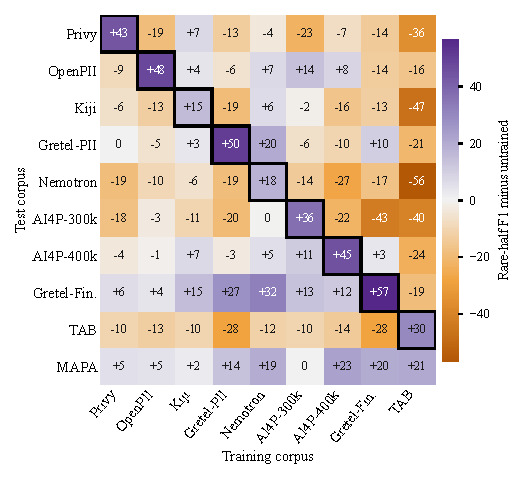
\includegraphics[width=\columnwidth]{figs/paper/fig_transfer.pdf}
\caption{GLiNER2 trained on one corpus (columns), evaluated on every test
set (rows): rare-half F1 minus the untrained model's. Outlined: the
training corpus. Scores are in Table~\ref{tab:transfer}.}
\label{fig:transfer}
\end{figure}

\subsection{A controlled transfer test}
\label{sec:transfer}

We train GLiNER2 with objective (b) (seed 42) on each of \tm{homes}
synthetic corpora and on TAB, and evaluate every model on all ten
(Figure~\ref{fig:transfer}); the hypotheses and the reading rule were
fixed before the runs. Each synthetic model ranks first on its own
corpus among all \tm{nsystems} systems, and its median rank elsewhere
falls to \tm{rankmin}--\tm{rankmax}. On the other corpora,
\tm{belowbase} of the \tm{homes} models score below the same model
without training (median difference \tm{gainmin} to \tm{gainmax}); the
two exceptions were trained on the corpora with the most languages
(Kiji) and the most types (Nemotron-PII). Every re-evaluated checkpoint
reproduces its original predictions exactly.

\paragraph{A human-annotated corpus does the same.}
If the effect came from synthetic generators, a model trained on human
annotation would escape it. It does not. Trained on TAB, GLiNER2 scores
\rv{tabhome} on TAB against \rv{tabnext} for the best other system,
ranks last elsewhere (median \rv{tabmedrank} of \rv{tabnsys}), and falls
below the untrained model on \rv{tabbelow} of \rv{tabnelse} other
corpora; its one gain is on MAPA, the other human-annotated legal
corpus. By the rule fixed beforehand, the effect belongs to training on
one corpus, not to synthetic data.

\subsection{Why trained models lose elsewhere}
\label{sec:names}

A model can lose on another corpus because it stops predicting some
types, because it has forgotten how to read type names it was not
trained on, or because the domain differs. Collapse explains little:
of the \rv{below} (model, corpus) pairs where a synthetic model falls
below the untrained one, only \rv{belowzero} have more types with no
prediction, and on the rare types both models predict, the median
difference is still \rv{dboth}. The training schema explains more.
Median recall falls from \rv{shareduntrained} to \rv{sharedtrained} on
types that also exist in the training schema, but from
\rv{unseenuntrained} to \rv{unseentrained} on the others; the TAB model
shows the same split. In this split a type and its name go together, so
it cannot tell whether the model lost the type or only its name.

\paragraph{Renaming types does not hurt a trained model.}
We therefore renamed every type at test time to its own description,
kept the description, and mapped predictions back before scoring
(Table~\ref{tab:labelpara} in Appendix~\ref{app:zeroshot}). On its own
corpus, a trained model barely changes (median \lp{dtrained}, at worst
\lp{dtrainedmin}), while the untrained model changes by a median of
\lp{duntrained} (\lp{duntrainedmin} to \lp{duntrainedmax}). We had
predicted that renaming would hurt the trained model more than the
untrained one on at least seven of nine corpora; the difference went
that way on \lp{didneg} ($p=\lp{p}$; on micro-F1, \lp{microneg} with
$p=\lp{microp}$), so the prediction is not met. The trained models are
not tied to the strings they were trained with, and their loss
elsewhere is better explained by the types their schema lacks than by
unfamiliar names.

\paragraph{Names matter for models not trained on the corpus.}
The untrained model, by contrast, moved with the names. We therefore
asked, with a protocol fixed before the runs, how a practitioner should
name the types when using a model without training on the target corpus.
For GLiNER2 Multi-v1 and the released GLiNER2-PII, we compared three
deterministic namings on each corpus's validation split: the original
names, the names in lower case with spaces (\texttt{ACCOUNT\_NUMBER}
$\to$ \emph{account number}), and the type's description. The naming
that won on validation raised rare-half F1 on test on \nm{un@improved}
of \nm{un@n} corpora for both models (median \nm{un@gain}, $p=\nm{un@p}$;
and \nm{pii@gain}, $p=\nm{pii@p}$; Table~\ref{tab:naming}). The
description won on most corpora; the lower-cased names won where the
original names were already words joined by underscores. Using the
description everywhere, without validation, still helps on
\nm{un@globalimproved} and \nm{pii@globalimproved} of 9 corpora. The
only loss was on OpenPII.

\subsection{A model not trained on the audited corpora}
\label{sec:zeroshot}

GLiNER2 Multi-v1 without training was not trained on these corpora's
released splits, although we cannot verify that its training data
excludes their generators (Appendix~\ref{app:zeroshot}). It reproduces
the few-mention effect: a support floor of ten changes its rare-half
score by \zs{kiji}{floorshift} on Kiji and \zs{gretel}{floorshift} on
Gretel-PII. It also shows that repeated values are not simply easier
for a trained model. Training widens the recall gap between repeated
and novel values on \zs{all}{pooledpos} of \zs{all}{didn} corpora when
types are pooled, but only on \zs{all}{didpos} within types, so most of
the pooled gap is a composition effect.

% =====================================================================
\section{Discussion}
\label{sec:discussion}

The flaws an audit finds are real, and correcting for them barely moves
rankings. That is good news for comparisons on a single corpus: its
leaderboard is not an artifact of how it is scored. It is bad news for
what the leaderboard means. A system trained on the corpus's own split
wins it, and the same model loses elsewhere, whether the corpus is
synthetic or written by people. Its loss tracks the types its training
schema lacks, and it does not depend on what the types are called. A PII
benchmark with a
public training split therefore measures, to a large extent, fit to
that split. Reporting one corpus or one metric, or omitting what a
system was trained on, turns that fit into an apparent quality of the
system. The same caution applies to training methods: a gain from one
objective rested on a single two-mention type, which only a support
floor exposes.

% =====================================================================
\section{Recommendations}
\label{sec:recommendations}

\begin{enumerate}
\item \textbf{Compare systems on several corpora, and state what each
was trained on.} Every model trained on a corpus won it, and most lost
elsewhere.
\item \textbf{Report test support with every per-type score}, a
rare-type average without types under ten test mentions, and micro-F1
next to it: the two named different best systems on most corpora.
\item \textbf{Report a novel-value score, compared within types.}
Pooled comparisons of repeated and novel values mix types.
\item \textbf{Audit a corpus before using it} for unfilled slots,
offsets that do not reproduce values, and PII outside the schema. The
released toolkit runs every probe without a model.
\item \textbf{Choose type names on validation} when a model is used
without training on the target corpus: on our corpora this raised
rare-type F1 by a median of \nm{un@gain} to \nm{pii@gain} points.
\item \textbf{Treat training runs as the unit of variation.} Seeds of
one objective differed by up to \rt{cgretelspread} points on one
corpus, which a sentence-level bootstrap does not see.
\end{enumerate}

% =====================================================================
\section{Conclusion}
\label{sec:conclusion}

Public PII corpora contain thinly tested rare types, values repeated
from training, and, in a few cases, generator artifacts and schema
gaps. Correcting for them moves scores but reorders only systems that
are already close. What decides a PII benchmark's ranking is whether a
system was trained on the benchmark's own split: every model trained on
one corpus wins it and usually loses elsewhere, on synthetic and
human-annotated corpora alike, and it loses most on the types its
schema lacks. A model not trained on the corpus depends instead on how
its types are named, and choosing names on validation is a cheap gain. PII detectors should be
compared on several corpora and metrics, with their training data
disclosed.

\FloatBarrier
\section*{Limitations}

The probes are automatic, and the check of how many flags are real
was done by an LLM, not by people; its passes agree with each other,
which does not rule out errors they share. U covers only five types that
patterns can validate. All systems are GLiNER-family extractors, chosen
because they accept any schema; we do not know whether fixed-label
taggers, rule systems, or prompted LLMs behave the same, and the naming
results concern models that read type names. The transfer test uses
one seed per training corpus and a single human-annotated control. It
does not include mixtures of corpora, so it cannot separate a missing
type from a missing domain, and the renaming test uses one paraphrase,
the type's own description. The naming study covers two GLiNER2 models
and three deterministic namings.
Comparisons of objectives rest on four corpora, too few for a
corpus-level test to reach significance, and the rank correlations of
released systems on five systems. Released systems are evaluated once, at a
fixed threshold, and GLiNER v1
checkpoints receive type descriptions rather than the label names they
were trained with. Only two released systems were trained on an audited
corpus. Objectives (a) and (c) have two seeds and (b)
three; the ablation has two. The rare half is defined by test support, which is itself
an audited property (Appendix~\ref{app:per_corpus}), and the merging rule
of V3 is coarse.

\section*{Ethics Statement}

We analyze publicly released corpora and do not attempt to identify
individuals. The examples quoted come from synthetic corpora; from TAB
and MAPA we report only aggregate statistics and generic strings such as
country names. PII detection is privacy sensitive, and a detector chosen
by a benchmark it was trained on may miss PII its training corpus never
labeled. Dataset use follows the licenses of the original releases.

\bibliographystyle{acl_natbib}
\bibliography{acl2027,rare_pii_extra,pii_audit_extra}

\appendix

\FloatBarrier
\section{Protocol and Deviations}
\label{app:protocol}

The protocol fixed the three objectives and their settings, the seeds,
the threshold rule, the primary endpoint ((c)$-$(b) on rare-half
macro-F1), and the decision rule before any run of (b). It was written
after an earlier comparison of (a) and (c) (Appendix~\ref{app:pilot}).
Every deviation is logged with its date and reason in the released
protocol file. The protocol is not registered with a third party. Its
first commit to version control postdates the runs of (b); it precedes
the runs of the added analyses of this version (the trained runs on
AI4Privacy, the ablation, and the off-the-shelf systems). The main ones are:
\begin{itemize}
\item The budget limited the runs to seeds 42 and 1337 for all three
objectives, plus seed 2024 for (b). A seed enters an objective's average
only once it exists on all four corpora.
\item The deciding test was changed from a sentence-level bootstrap to
the run-level sign-flip test before any seed-2024 run finished. The
bootstrap gave $+0.45$ $[-0.10,+0.78]$ for (c)$-$(b) on seeds 42 and
1337 and is still reported.
\item The audit (Section~\ref{sec:audit}) and the re-scoring variants
(Section~\ref{sec:consequences}) were added after the first results.
They are exploratory. The variants and their reading rule were written
before they were computed. The zero-shot analyses of
Section~\ref{sec:zeroshot} were also written before the runs; the
within-type comparison was added after the pooled result was seen.
The zero-shot run on Gretel-Finance first failed silently: the evaluator
recorded an out-of-memory error on 4{,}900 of 5{,}000 documents as empty
predictions. It was rerun one document at a time; one document still
failed and is excluded. No run of objectives (a)--(c) has a failed
document. The same document failed for GLiNER2-PII and is excluded there.
\item The first trained runs on AI4Privacy-300k skipped 94--135
batches each on out-of-memory errors, which silently drops the heaviest
documents. They were cancelled and rerun on a 40\,GB A100 with micro-batch
4 and accumulation 4 (the effective batch is unchanged), with a guard
that stops a run at the first skipped batch or NaN loss; the reruns
skipped none. The Nemotron-PII and Gretel-Finance models of the transfer
test needed an 80\,GB A100 for the same reason. The ten Gretel GLiNER
runs first failed on a stale deployment and were rerun unchanged.
\item An ablation run on OpenPII (A10G, micro-batch 8) skipped batches,
which raised the question whether the unguarded runs of objective (b)
had too. Re-running (b) with seed 42 on OpenPII and Kiji in that exact
configuration, counting rather than stopping, found no skipped batch and
no NaN loss; other seeds were not re-run.
\item Two checkpoints of the transfer test were first corrupted in a
download that preserved file sizes; the check that each checkpoint
reproduces its own run's predictions caught it. They were re-transferred
until two downloads agreed, after which the check passed.
\item The GLiNER2 trainer truncates texts at 2{,}048 words, which would
have dropped 11\% of TAB's training spans. The TAB models were trained
on TAB training and validation documents cut into pieces of at most
1{,}000 words at line breaks, never inside a span; no span was lost, and
the TAB test split is unchanged. This was fixed before the TAB runs, as
were the TAB control of Section~\ref{sec:transfer} and the label-name
intervention of Section~\ref{sec:names}, both added in response to an
earlier review.
\end{itemize}
Because the earlier runs kept only candidates scored at least $0.5$,
tuned thresholds are searched in \tuneGrid{} by filtering the decode at
$0.5$. This equals re-decoding when conflicts are resolved by score. We
verified the equality on dry-run sentences.

\FloatBarrier
\section{Probe Details and Sources}
\label{app:probes}

\paragraph{Sources.}
All corpora are on the Hugging Face Hub (Table~\ref{tab:sources}).
Gretel-Finance ships the same documents three times (per language,
combined, and the default configuration); we use the default one.

\begin{table}[h]
\centering
\footnotesize
\setlength{\tabcolsep}{3pt}
\begin{tabular}{@{}ll@{}}
\toprule
Corpus & Hub identifier \\
\midrule
Privy & \texttt{piimb/privy} \\
OpenPII & \texttt{ai4privacy/open-pii-masking-500k-}\\
 & \quad\texttt{ai4privacy} \\
Kiji & \texttt{DataikuNLP/kiji-pii-training-data} \\
Gretel-PII & \texttt{gretelai/gretel-pii-masking-en-v1} \\
Nemotron-PII & \texttt{nvidia/Nemotron-PII} \\
AI4Privacy-300k & \texttt{ai4privacy/pii-masking-300k} \\
AI4Privacy-400k & \texttt{ai4privacy/pii-masking-400k} \\
Gretel-Finance & \texttt{gretelai/synthetic\_pii\_finance\_}\\
 & \quad\texttt{multilingual} \\
TAB & \texttt{ildpil/text-anonymization-}\\
 & \quad\texttt{benchmark} \\
MAPA & \texttt{piimb/mapa-eur-lex-pii} \\
\bottomrule
\end{tabular}
\caption{Sources of the audited corpora.}
\label{tab:sources}
\end{table}

\paragraph{Implementation.}
Templates replace each gold span by its type in angle brackets, replace
digits by 0, lower-case, and collapse whitespace; overlapping spans keep
the first. U uses the regex and checksum validators of our rule-based
detector. A hit counts as covered if any gold span overlaps it. The
schema has a type for it if a type name matches the rule type (e.g.
\textsc{ipv4} for IP). G matches bracketed upper-case tokens of at least
four characters, \texttt{\{\{\ldots\}\}}, and generator markup of the
form \texttt{NAME\_XX(}. Bracketed log levels (\texttt{[ERROR]},
\texttt{[INFO]}, \ldots) are excluded, after they appeared as false
alarms in Nemotron-PII and Gretel-Finance. For TAB, the probes other than IAA
use one annotator per document (the first by annotator id).

\FloatBarrier
\section{Model Review of the Probe Flags}
\label{app:validation}

\begin{table}[h]
\centering
\small
\setlength{\tabcolsep}{3pt}
\resizebox{\columnwidth}{!}{%
\begin{tabular}{@{}llrrlrr@{}}
\toprule
Corpus & Probe & Flags & Sampled & Real \% [95\% CI] & Fleiss $\kappa$ & Est. real \\
\midrule
\genrows{tab_validation_body}
\bottomrule
\end{tabular}%
}
\caption{Model review per corpus and probe: share of sampled flags
judged real by the majority of three passes (Wilson 95\% CI), and that
share applied to all flags of the cell. --: all answers identical.}
\label{tab:validation_full}
\end{table}

\begin{table*}[h]
\centering
\small
\setlength{\tabcolsep}{4pt}
\begin{tabular}{@{}l l l p{0.62\textwidth}@{}}
\toprule
Probe & Corpus & Gold & Excerpt (flagged text in bold) \\
\midrule
G & AI4Privacy-400k & -- & Dag [NAME\_1], willen we het bedrag van \textbf{[AMOUNT\_1]} betwisten. \\
G & Nemotron-PII & -- & STATE OF \textbf{[STATE]} \quad COUNTY OF [COUNTY] \quad AFFIANT: \ldots \\
O & AI4Privacy-300k & \textsc{idcard} & value \texttt{UUL858997U, LASTNAME1\_F(Leivadas}; the offsets select \textbf{UUL858997U, Leivadas, Maggiolini} \\
C & AI4Privacy-300k & \textsc{time} & "Password": "b]Yh,L7", "Time": "\textbf{missing}", "Lastname": "missing" \\
C & Gretel-Finance & \textsc{company} & Vi vill ge \textbf{[Organisationsnamn]} vår högsta rekommendation \ldots \\
U & AI4Privacy-400k & -- & Diamond Bar claim payment is pending. Visit \textbf{http://www.oconnor.com/}, confirm 2746. \\
\bottomrule
\end{tabular}
\caption{Flags that all three review passes judged real problems: unfilled
slots (G), offsets that select other text (O), null tokens and slots
labeled as entities (C), and PII the schema has no type for (U).
Examples are from synthetic corpora only.}
\label{tab:flag_examples}
\end{table*}

Table~\ref{tab:flag_examples} shows flags judged real by all three
passes. Items were drawn with a fixed seed, at most 20 per corpus and probe,
then topped up to at most 50 with a second seed from the remaining
flags of each cell, after the first 435 had been judged; the shares
on the first 435 alone differ from those reported by at most 2.5
points per probe. Items are shuffled across cells. Each item shows the flagged text in 90 characters
of context. Each pass answers from the closed set per probe that the
released sheet lists (O: harmful/benign; C: wrong/legitimate; U: missed
in-schema/outside the schema/not PII; G: artifact/text; each with
``unclear''). The three passes are separate runs of one model with no
access to each other's answers, to the corpus name, or to code; each
sees the items in a different random order. An item's label is the
answer of at least two passes; items without a majority, or with
``unclear'' as the majority, are dropped from the share. Agreement
between passes measures the consistency of one model, not
inter-annotator agreement, and a model may share systematic errors
across passes. The decision to replace the planned two-person check
was recorded before any answer was read (PROTOCOL.md 9.16); the three
answer sheets are released.

\FloatBarrier
\section{Training-Objective Contrasts}
\label{app:contrasts}

Table~\ref{tab:contrasts} gives the contrasts between the three objectives at the tuned
threshold, and Table~\ref{tab:sensitivity} re-scores them under the variants of
Section~\ref{sec:consequences}.

\begin{table*}[h]
\centering
\small
\setlength{\tabcolsep}{5pt}
\begin{tabular}{@{}lcc cc cc c@{}}
\toprule
& & Test sentences & \multicolumn{2}{c}{Training runs} & \multicolumn{2}{c}{Rare labels} & \\
\cmidrule(lr){3-3}\cmidrule(lr){4-5}\cmidrule(lr){6-7}
Contrast & $\Delta$ Rare-half & 95\% CI (bootstrap) & $p$ (sign-flip) & runs $>0$
& labels $>0$ & $p$ (Wilcoxon) & $\Delta$ Macro / Micro \\
\midrule
\genrows{tab_tests_body}
\bottomrule
\end{tabular}
\caption{Contrasts between objectives at the tuned threshold, mean of
four corpora, seeds 42 and 1337. Primary endpoint: (c)$-$(b).}
\label{tab:contrasts}
\end{table*}

\begin{table*}[h]
\centering
\small
\setlength{\tabcolsep}{4.5pt}
\begin{tabular}{@{}l ccc ccc ccc@{}}
\toprule
& \multicolumn{3}{c}{Rare-half macro-F1} & \multicolumn{3}{c}{(b)$-$(a)} & \multicolumn{3}{c}{(c)$-$(b)} \\
\cmidrule(lr){2-4}\cmidrule(lr){5-7}\cmidrule(lr){8-10}
Variant & (a) & (b) & (c) & $\Delta$ & $p$ & runs $>0$ & $\Delta$ & $p$ & runs $>0$ \\
\midrule
\genrows{tab_sensitivity_body}
\bottomrule
\end{tabular}
\caption{Objectives re-scored under each variant (thresholds fixed;
seeds 42 and 1337). $p$: sign-flip over eight (corpus, seed) pairs. No
type has 10--19 mentions, so V1-10 and V1-20 coincide.}
\label{tab:sensitivity}
\end{table*}

\section{Ablation of Negative Masking}
\label{app:ablation}

Objective (b) differs from (a) in several components, one of which is
that it keeps every negative span--type cell. To check whether dropping
the masking alone explains the gain, (a$'$) is (a) with masking switched
off and nothing else changed (Table~\ref{tab:ablation}). The reading
rule, fixed before the runs, called masking the main source of the gain
if (a$'$)$-$(a) reached half of (b)$-$(a). It does not: averaged over
seeds 42 and 1337 the masking alone gives \ab{fa} points against
\ab{ba} for (b), and it is negative on OpenPII
(\ab{pii_500k@fa}), where (b) gains most.

\begin{table}[h]
\centering
\small
\setlength{\tabcolsep}{5pt}
\begin{tabular}{@{}lrr@{}}
\toprule
Corpus & (a$'$)$-$(a) & (b)$-$(a) \\
\midrule
Privy & \ab{privy@fa} & \ab{privy@ba} \\
OpenPII & \ab{pii_500k@fa} & \ab{pii_500k@ba} \\
Kiji & \ab{kiji@fa} & \ab{kiji@ba} \\
Gretel-PII & \ab{gretel@fa} & \ab{gretel@ba} \\
\midrule
Mean & \ab{fa} & \ab{ba} \\
\bottomrule
\end{tabular}
\caption{Ablation: (a$'$) is (a) with negative masking off and
nothing else changed (rare-half macro-F1 differences).}
\label{tab:ablation}
\end{table}

\FloatBarrier
\section{Objective Details}
\label{app:objectives}

\begin{table}[h]
\centering
\small
\setlength{\tabcolsep}{5pt}
\begin{tabular}{@{}lccc@{}}
\toprule
Component & (a) & (b) & (c) \\
\midrule
Per-cell BCE & \yes & \yes & \yes \\
Negative masking ($p=0.5$) & \yes & \no & \no \\
Class weights & \no & \yes & \yes \\
Positive weight $w_{+}=2$ & \no & \yes & \yes \\
Boundary smoothing $\epsilon=0.1$ & \no & \yes & \yes \\
Learned per-type operating point & \no & \yes & \yes \\
Span, type ranking; active negatives & \no & \no & \yes \\
\bottomrule
\end{tabular}
\caption{Components of the three nested objectives.}
\label{tab:objectives}
\end{table}


For type $\ell$ let $s_{c,\ell}$ be the logit of span $c$, shifted so
that $s_{c,\ell}>0$ exactly when the span is active. Let
$\mathcal{T}_\ell$ be the active spans, and let $\mathcal{G}_\ell$ be
the gold spans. An active non-gold span $c\in\mathcal{T}_\ell\setminus\mathcal{G}_\ell$
whose highest IoU with a gold span of type $\ell$ is at least $\tau$ is a
boundary rival of that span $g$, and these rivals form $\mathcal{O}(g)$;
active non-gold spans whose highest IoU is below $\tau$ form $\mathcal{F}_\ell$. Objective (c)
adds
\begin{align*}
\mathcal{L}_{\mathrm{span}}&=\textstyle\sum_{g}\,[m+\max_{c\in\mathcal{O}(g)}s_{c,\ell_g}-s_{g,\ell_g}]_+,\\
\mathcal{L}_{\mathrm{type}}&=\textstyle\sum_{g}\,[m+\max_{\ell'\neq\ell_g}s_{g,\ell'}-s_{g,\ell_g}]_+,\\
\mathcal{L}_{\mathrm{fp}}&=\textstyle\sum_{\ell}\sum_{c\in\mathcal{F}_\ell}\mathrm{softplus}(s_{c,\ell}),
\end{align*}
with weights $1$, $0.25$, $0.25$, margin $m=0.5$, and $\tau=0.5$, fixed
before the experiments. $\mathcal{L}_{\mathrm{fp}}$ raises the weight of
each active unmatched negative from $1$ to $1.25$.

\FloatBarrier
\section{PII Preprocessing of the Case-Study Corpora}
\label{app:pii_preprocessing}

All annotations are converted to character spans, and every span is
checked against the text. Privy labels every non-Presidio span as
outside, including real e-mail addresses and URLs, so its 17-type schema
is what was annotated, not every PII mention. Its text field is a byte
string representation, and gold offsets refer to that string, so we keep
it. Training documents longer than 2{,}000 characters (78) are removed.
Gretel-PII provides entity strings without offsets. We recover offsets
by exact search; on 5{,}000 rows no string was missing or ambiguous.
When two annotations overlap, the longer is kept. Kiji and OpenPII
lack a validation split of the needed size, so validation is carved from
the tail of an upstream split. Types with fewer than 20 training mentions
are removed.

\FloatBarrier
\section{Implementation Details}
\label{app:implementation}

All models are trained with the GLiNER2 trainer from
\texttt{fastino/gliner2-multi-v1} (Table~\ref{tab:implementation}).
Corpora whose longest documents ran out of memory on an A10G were moved
to larger GPUs at a smaller micro-batch with the same effective batch
of 16, and every run after the first AI4Privacy-300k attempt is stopped
at the first skipped batch or NaN loss (Appendix~\ref{app:protocol}).
Evaluation uses the type descriptions with the registry's casing,
threshold 0.5 unless stated otherwise, greedy flat decoding that keeps
the higher-scoring of two overlapping spans, and documents cut into
chunks of at most 2{,}048 words. The \cb{runs} runs recorded by our runner used \cb{total} GPU hours:
\cb{aten} on A10G, \cb{afour} on A100 40GB, \cb{aeight} on A100 80GB,
and \cb{h} on H200, of which \cb{evalonly} were evaluation without
training. This is a lower bound: it excludes about \cb{smoke} hours of
smoke tests and runs stopped before they wrote a record. Scores use
strict matching: a
prediction counts only with the exact boundaries and type of a gold
span, paired one-to-one by the Hungarian algorithm.

\begin{table}[h]
\centering
\small
\renewcommand{\arraystretch}{1.1}
\begin{tabular}{p{0.36\linewidth} p{0.52\linewidth}}
\toprule
Setting & Value \\
\midrule
Initialization & \texttt{fastino/gliner2-multi-v1} \\
Hardware & A10G; A100 40GB (Gretel-PII, AI4Privacy-300k); A100 80GB (Privy, Nemotron-PII, Gretel-Finance); H200 (TAB) \\
Seeds & \seedList \\
Optimizer & AdamW \\
Learning rate & $1\times10^{-5}$ encoder, $5\times10^{-4}$ task layers \\
Schedule & linear, warm-up ratio $0.1$ \\
Epochs & 3 \\
Effective batch size & 16 ($8\times2$; $4\times4$ for the corpora with the longest documents) \\
Precision & FP16 (Privy: BF16) \\
\midrule
Class weights & inverse training frequency, capped at 10 \\
Positive weight & $w_{+}=2$ \\
Boundary smoothing & $\epsilon=0.1$, distance 1 \\
Null anchor & initialized at $p=0.7$ \\
\bottomrule
\end{tabular}
\caption{Training configuration of every trained model.}
\label{tab:implementation}
\end{table}

\FloatBarrier
\section{Per-Corpus Results}
\label{app:per_corpus}

Table~\ref{tab:main} gives the three objectives on each corpus, at the
fixed threshold and at the threshold tuned on validation; tuning moves
no average by more than 0.1 points. The objectives differ most on
Gretel-PII and OpenPII and barely on Privy, where every objective is
above 99. The large standard deviation of (c) on Gretel-PII (about 2
points) reflects the two-mention PIN type of Section~\ref{sec:case}.
Table~\ref{tab:per_corpus} gives macro- and micro-F1: macro-F1 follows
the rare-half pattern on a smaller scale, and micro-F1 differs between
objectives by at most 0.4 points on any corpus. Because the rare half is
itself defined by test support, an audited property,
Table~\ref{tab:rare_partition} redefines it by training frequency: the
two definitions agree on 89--95\% of types, and (c)$-$(b) changes by at
most 0.05 points.

\begin{table*}[h]
\centering
\small
\setlength{\tabcolsep}{4.5pt}
\resizebox{\textwidth}{!}{%
\begin{tabular}{@{}ll ccccc cc@{}}
\toprule
& & \multicolumn{5}{c}{Rare-half macro-F1} & Macro-F1 & Micro-F1 \\
\cmidrule(lr){3-7}\cmidrule(lr){8-8}\cmidrule(lr){9-9}
Threshold & Objective & Privy & OpenPII & Kiji & Gretel-PII & Avg & Avg & Avg \\
\midrule
\genrows{tab_main_body}
\bottomrule
\end{tabular}%
}
\caption{GLiNER2 on the four case-study corpora, mean $\pm$ standard
deviation over seeds (\seedList). Avg columns average the per-corpus
means.}
\label{tab:main}
\end{table*}

\begin{table*}[h]
\centering
\small
\setlength{\tabcolsep}{4pt}
\resizebox{\textwidth}{!}{%
\begin{tabular}{@{}ll cccc cccc@{}}
\toprule
& & \multicolumn{4}{c}{Macro-F1} & \multicolumn{4}{c}{Micro-F1} \\
\cmidrule(lr){3-6}\cmidrule(lr){7-10}
Threshold & Objective & Privy & OpenPII & Kiji & Gretel-PII & Privy & OpenPII & Kiji & Gretel-PII \\
\midrule
\genrows{tab_per_corpus_body}
\bottomrule
\end{tabular}%
}
\caption{Per-corpus macro- and micro-F1, mean $\pm$ standard deviation
over seeds.}
\label{tab:per_corpus}
\end{table*}

\begin{table}[h]
\centering
\small
\setlength{\tabcolsep}{4pt}
\begin{tabular}{@{}lccc@{}}
\toprule
Corpus & Test support & Train frequency & Overlap \\
\midrule
\genrows{tab_rare_partition_body}
\bottomrule
\end{tabular}
\caption{(c)$-$(b) with the rare half defined by test support or by
training frequency; overlap: share of labels both define as rare.}
\label{tab:rare_partition}
\end{table}

\FloatBarrier
\section{Where the Objectives Change Errors}
\label{app:errors}

Each gold span is classified as correct, a type error, a boundary error,
both, or missed, and each unmatched prediction as spurious
(Table~\ref{tab:error_change}, Figure~\ref{fig:per_corpus}). On the
low-support half, (b) turns type errors and spurious predictions into
correct ones (+0.68 points of gold correct, $-$0.56 type errors,
$-$0.40 spurious), at a small cost on the high-support half. (c)
changes every category by less than 0.15 points.

\begin{table}[h]
\centering
\small
\setlength{\tabcolsep}{3.5pt}
\begin{tabular}{@{}lrrrr@{}}
\toprule
& \multicolumn{2}{c}{(b)$-$(a)} & \multicolumn{2}{c}{(c)$-$(b)} \\
\cmidrule(lr){2-3}\cmidrule(lr){4-5}
\% of gold & Low & High & Low & High \\
\midrule
\genrows{tab_error_change_body}
\bottomrule
\end{tabular}
\caption{Change in errors between objectives at $p_0=0.5$, as \% of
gold support in each support half (four corpora pooled).}
\label{tab:error_change}
\end{table}

\begin{figure*}[h]
\centering
\IfFileExists{figs/paper/fig_rare_pii_errors.pdf}{%
  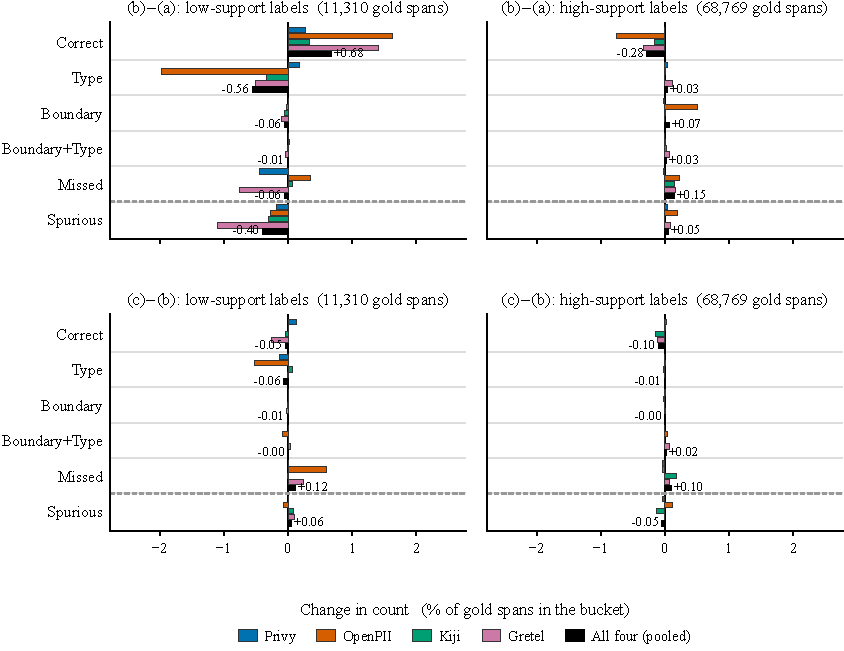
\includegraphics[width=\textwidth]{figs/paper/fig_rare_pii_errors.pdf}}{%
  \figpending{per-corpus error changes}}
\caption{Per-corpus error changes at $p_0=0.5$ (\% of gold spans per
support half). Black bars: the pooled values of
Table~\ref{tab:error_change}.}
\label{fig:per_corpus}
\end{figure*}

\FloatBarrier
\section{Transfer Matrix}
\label{app:transfer}

Table~\ref{tab:transfer} gives the scores behind Figure~\ref{fig:transfer}.

\begin{table*}[h]
\centering
\small
\setlength{\tabcolsep}{4pt}
\resizebox{\textwidth}{!}{%
\begin{tabular}{@{}l cccccccc c c@{}}
\toprule
& \multicolumn{9}{c}{GLiNER2 trained with objective (b) on} & \\
\cmidrule(lr){2-10}
Test corpus & Privy & OpenPII & Kiji & Gretel-PII & Nemotron & AI4P-300k & AI4P-400k & Gretel-Fin. & TAB & untrained \\
\midrule
\genrows{tab_transfer_body}
\bottomrule
\end{tabular}%
}
\caption{GLiNER2 trained on one corpus (columns) evaluated on every test
set (rows): rare-half macro-F1. Bold: the training corpus. The 0.0
cells: no prediction of TAB's four rarer types.}
\label{tab:transfer}
\end{table*}

\FloatBarrier
\section{GLiNER2 Without Training}
\label{app:zeroshot}

Table~\ref{tab:labelpara} gives the renaming test of
Section~\ref{sec:names} per corpus, Table~\ref{tab:naming} the namings
chosen on validation and their test scores, and Table~\ref{tab:zeroshot}
the untrained model on all ten test splits. In Table~\ref{tab:zeroshot}, a
support floor of ten raises the rare-half score only on the two corpora
with types under ten test mentions (Kiji and Gretel-PII); removing
predictions in flagged regions changes precision only on
AI4Privacy-400k, where they are 3.7\% of the false positives; and the
gap between repeated and novel values widens with training on most
corpora when types are pooled, but on fewer within types.

\begin{table}[h]
\centering
\small
\setlength{\tabcolsep}{3pt}
\resizebox{\columnwidth}{!}{%
\begin{tabular}{@{}l rrr rrr r@{}}
\toprule
& \multicolumn{3}{c}{Trained on the corpus} & \multicolumn{3}{c}{Untrained} & \\
\cmidrule(lr){2-4}\cmidrule(lr){5-7}
Corpus & names & renamed & $\Delta$ & names & renamed & $\Delta$ & DiD \\
\midrule
\genrows{tab_labelpara_body}
\bottomrule
\end{tabular}%
}
\caption{Renaming each type to its description at test time (rare-half
macro-F1 on the corpus's test split). DiD: trained $\Delta$ minus
untrained $\Delta$.}
\label{tab:labelpara}
\end{table}

\begin{table}[h]
\centering
\small
\setlength{\tabcolsep}{2.5pt}
\resizebox{\columnwidth}{!}{%
\begin{tabular}{@{}l lrrr lrrr@{}}
\toprule
& \multicolumn{4}{c}{GLiNER2 Multi-v1} & \multicolumn{4}{c}{GLiNER2-PII} \\
\cmidrule(lr){2-5}\cmidrule(lr){6-9}
Corpus & chosen & names & chosen & $\Delta$ & chosen & names & chosen & $\Delta$ \\
\midrule
\genrows{tab_naming_body}
\bottomrule
\end{tabular}%
}
\caption{Type names chosen on validation (original, lower case with
spaces, or description), scored on test: rare-half macro-F1 with the
original names and with the chosen ones.}
\label{tab:naming}
\end{table}

\begin{table*}[h]
\centering
\small
\setlength{\tabcolsep}{4pt}
\resizebox{\textwidth}{!}{%
\begin{tabular}{@{}l ccc cc ccc@{}}
\toprule
& \multicolumn{2}{c}{Rare-half macro-F1} & & \multicolumn{2}{c}{Flagged regions}
& \multicolumn{3}{c}{Trained minus zero-shot, seen$-$novel recall} \\
\cmidrule(lr){2-3}\cmidrule(lr){5-6}\cmidrule(lr){7-9}
Corpus & as scored & support $\geq 10$ & Micro-F1 & precision & \% of FP & pooled & within type & types $>0$ \\
\midrule
\genrows{tab_zeroshot_body}
\bottomrule
\end{tabular}%
}
\caption{GLiNER2 without training on the ten test splits.
\emph{Flagged regions}: precision before and after removing false
positives in flagged regions. \emph{Trained minus zero-shot}: change in
the recall gap between repeated and novel values after training with
(b), pooled and within types ($\geq$20 mentions each); --: no training
split.}
\label{tab:zeroshot}
\end{table*}

\FloatBarrier
\section{Provenance of Objectives (a) and (c)}
\label{app:pilot}

Objectives (a) and (c) were first compared on the four corpora with
seeds 42 and 1337, before the protocol was written. There, (c) raised
rare-half macro-F1 over (a). But (c) differs from (a) in several
components at once, so that comparison could not say which of them mattered;
this motivated objective (b). The same runs are the (a) and (c) rows of
Table~\ref{tab:main}.

\end{document}
